\documentclass[11pt,a4paper]{article}

\usepackage[T1]{fontenc}
\usepackage[utf8]{inputenc}
\usepackage[a4paper,margin=2.5cm]{geometry}
\usepackage{microtype}
\usepackage{etoolbox}
\usepackage{setspace}
\usepackage{graphicx}
\usepackage{booktabs}
\usepackage{tabularx}
\usepackage{longtable}
\usepackage{array}
\usepackage{amsmath,amssymb}
\usepackage{enumitem}
\usepackage{caption}
\usepackage{xcolor}
\usepackage{fancyhdr}
\usepackage{titlesec}
\usepackage{cite}
\usepackage[hidelinks]{hyperref}
\usepackage[nameinlink,noabbrev]{cleveref}
\usepackage{placeins}

\definecolor{ink}{HTML}{20303C}
\definecolor{muted}{HTML}{5A6975}
\definecolor{rulegray}{HTML}{AAB4BC}
\definecolor{reportblue}{HTML}{2F6B8A}
\definecolor{reportred}{HTML}{A44F39}

\hypersetup{
  pdfauthor={Adit Patil},
  pdftitle={Bundle Neural Networks for Functional Connectomes},
  pdfsubject={Completed research report with accepted-checkpoint mechanism audit},
  pdfkeywords={ABIDE-I, functional connectome, bundle neural network, graph neural network}
}

\setstretch{1.5}
\setlength{\parindent}{1.5em}
\setlength{\parskip}{0.15em}
\setlength{\emergencystretch}{2em}
\setlist{itemsep=0.2em,topsep=0.4em}
\captionsetup{font={small,stretch=1.0},labelfont=bf,skip=6pt}
\AtBeginEnvironment{table}{\singlespacing}
\AtBeginEnvironment{longtable}{\singlespacing}
\titleformat{\section}{\Large\bfseries\color{ink}}{\thesection}{0.7em}{}
\titleformat{\subsection}{\large\bfseries\color{ink}}{\thesubsection}{0.7em}{}
\titleformat{\subsubsection}{\normalsize\bfseries\color{ink}}{\thesubsubsection}{0.7em}{}
\pagestyle{fancy}
\fancyhf{}
\fancyhead[L]{\small Bundle Neural Networks for Functional Connectomes}
\fancyhead[R]{\small Completed evidence report}
\fancyfoot[C]{\thepage}
\renewcommand{\headrulewidth}{0.4pt}
\setlength{\headheight}{14pt}
\graphicspath{{../generated/figures/}{generated/figures/}}
\newcolumntype{Y}{>{\raggedright\arraybackslash}X}
\newcolumntype{R}{>{\raggedleft\arraybackslash}p{2.2cm}}
\newcommand{\ASD}{autism spectrum disorder}
\newcommand{\ABIDE}{Autism Brain Imaging Data Exchange}
\newcommand{\BuNN}{Bundle Neural Network}
\newcommand{\GCN}{Graph Convolutional Network}
\newcommand{\BA}{balanced accuracy}
\newcommand{\draftnote}{\textbf{Completed evidence draft.} This version reports the frozen ABIDE-I operator study and a separately labelled, audited post-hoc intervention analysis of its accepted BuNN checkpoints. External validation and additional architecture studies are not presented as completed results.}
% Generated by scripts/build_manuscript_inputs.py; do not edit manually.
\providecommand{\StudyParentRows}{769}
\providecommand{\StudyTechnicalExclusions}{15}
\providecommand{\StudyParticipants}{754}
\providecommand{\StudySites}{18}
\providecommand{\StudyASD}{371}
\providecommand{\StudyControls}{383}
\providecommand{\StudyROIs}{116}
\providecommand{\StudyEdges}{6,670}
\providecommand{\CovariatesBA}{0.5652}
\providecommand{\ConnectomeBA}{0.6401}
\providecommand{\CombinedBA}{0.6336}
\providecommand{\BunnGcnEstimate}{-0.00958}
\providecommand{\BunnGcnCILow}{-0.03665}
\providecommand{\BunnGcnCIHigh}{0.01146}
\providecommand{\BunnGcnP}{0.524}
\providecommand{\PracticalMargin}{0.03}
\providecommand{\BunnElasticEstimate}{-0.05516}
\providecommand{\BunnElasticCILow}{-0.08297}
\providecommand{\BunnElasticCIHigh}{-0.02752}
\providecommand{\BunnElasticP}{0.0018}
\providecommand{\RankEstimate}{-0.00719}
\providecommand{\RankCILow}{-0.01310}
\providecommand{\RankCIHigh}{-0.00105}
\providecommand{\LeaveOneSitePositive}{1}
\providecommand{\SeedPositive}{2}
\providecommand{\FavorableIntervals}{0}
\providecommand{\UnfavorableSeedIntervals}{1}
\providecommand{\GcnParameters}{5,889}
\providecommand{\BunnParameters}{8,529}
\providecommand{\GcnFitHours}{15.09}
\providecommand{\BunnFitHours}{31.14}
\providecommand{\GcnCurveBA}{0.5945}
\providecommand{\BunnCurveBA}{0.5849}


\begin{document}
\hypersetup{pageanchor=false}

% ---------------------------------------------------------------------------
% Cover
% ---------------------------------------------------------------------------
\thispagestyle{empty}
\begin{center}
  {\Large\bfseries Research Report}\par
  \vspace{0.35em}
  {\large 2026 S.T. Yau High School Science Award (Asia)}\par
  \vspace{2.0cm}
  {\LARGE\bfseries Bundle Neural Networks for Functional Connectomes}\par
  \vspace{0.35em}
  {\Large Density-Dependent Aggregation and Cross-Site Prediction}\par
  \vspace{1.2cm}
\end{center}

\renewcommand{\arraystretch}{1.35}
\noindent\begin{tabularx}{\textwidth}{|>{\bfseries\raggedright\arraybackslash}p{3.6cm}|Y|}
\hline
Team Member & Adit Patil \\
\hline
School & School of Scholars \\
\hline
City and Country & Akola, India \\
\hline
Registration Number & Comp-183 \\
\hline
Supervising Teacher & Anjali Tupe \\
\hline
Position & Class Teacher \\
\hline
Supervising School & School of Scholars, Akola, India \\
\hline
Report Version & Completed evidence report with E1 mechanism audit, 14 August 2026 \\
\hline
\end{tabularx}

\vfill
\noindent\begin{minipage}{\textwidth}
\small\color{muted}
\draftnote

This document is a separate report-format rendering. It does not replace the
existing IEEE-style manuscript. Before any actual submission, the researcher
must independently revise the prose, complete the acknowledgments and AI-use
disclosure, verify all personal details, and sign the integrity commitments.
\end{minipage}
\clearpage

% ---------------------------------------------------------------------------
% Front matter
% ---------------------------------------------------------------------------
\pagenumbering{roman}
\hypersetup{pageanchor=true}
\setcounter{page}{1}
\section*{Abstract}
\addcontentsline{toc}{section}{Abstract}

Functional connectomes have a natural graph representation, but the usual
node feature is already a complete connectivity profile. Neighborhood
aggregation may therefore blur useful differences instead of supplying new
information. This study tested whether learned orthogonal bundle transport
changes that density-dependent behavior. The analysis used
\StudyParticipants{} technically eligible ABIDE-I participants from
\StudySites{} sites. A shared neural backbone was paired with identity
propagation, a learned-local capacity control, Graph Convolutional Network
(GCN) aggregation, trivial-bundle diffusion, or learned Bundle Neural Network
(BuNN) transport. Nonzero graphs retained the strongest positive edges at 1,
5, 10, and 20 percent density. Evaluation used nested held-out-site validation,
five final seeds, regularized non-graph baselines, and common-frame
representation diagnostics.

The primary BuNN-minus-GCN performance-curve contrast was
\BunnGcnEstimate{} (95\% site-bootstrap confidence interval
[\BunnGcnCILow{}, \BunnGcnCIHigh{}]; exact sign-flip
$p=\BunnGcnP$). Relative to the connectome elastic net, the BuNN contrast was
\BunnElasticEstimate{} (95\% confidence interval
[\BunnElasticCILow{}, \BunnElasticCIHigh{}]). The matched-anchor
effective-rank contrast was \RankEstimate{} (95\% confidence interval
[\RankCILow{}, \RankCIHigh{}]), which ran against the proposed
representation-preservation advantage. Performance declined as graph density
increased for each diffusion operator. Site weighting and training seed also
affected the small BuNN--GCN difference.

A separately frozen post-hoc intervention analysis then tested what the 360
accepted BuNN checkpoints actually used. Replacing learned maps with random
orthogonal maps reduced equal-site balanced accuracy by 8.86 percentage
points (95\% interval $[-12.36,-4.78]$; Holm-adjusted exact
$p=0.0038$). Identity maps, shuffled learned maps, and degree-preserving graph
rewiring caused smaller reductions and did not pass the four-contrast
multiplicity-controlled test. Representation changes were substantial but
only weakly associated with prediction changes across site-density cells.

Under this specified ABIDE-I pipeline, learned bundle transport provided no
detected advantage over GCN or the elastic net. The intervention audit shows
that its learned maps nevertheless influenced its own predictions; the exact
graph topology contributed much less. The study does not establish a
biological bundle geometry, a clinical diagnostic system, or a universal
result for BuNNs. Its contribution is a controlled operator comparison and a
checkpoint-level audit in a dense, globally informed connectome setting.

\noindent\textbf{Keywords:} functional connectome; bundle neural network;
graph neural network; representation collapse; held-out-site validation;
ABIDE-I; autism

\clearpage
\section*{Acknowledgments and Assistance Statement}
\addcontentsline{toc}{section}{Acknowledgments and Assistance Statement}

The study used public, anonymized ABIDE-I derivatives distributed through the
Preprocessed Connectomes Project. The original ABIDE investigators and
participating institutions collected and shared those data; they were not
involved in the present analysis. The computational work used open-source
Python, PyTorch, NumPy, pandas, scikit-learn, and scientific plotting tools,
with training performed on an AWS EC2 instance equipped with an NVIDIA A10G
GPU.

AI systems assisted with literature discovery, protocol criticism, code
development and debugging, run monitoring, analysis checks, figure and table
production, and document formatting. The project maintains a dated local
record in \texttt{docs/ai\_use\_log.md}. AI assistance does not establish
authorship or responsibility for the scientific claims. Before external
submission, the student researcher must verify the analysis, rewrite or edit
the report in their own voice, and complete any missing tool versions, dates,
frequencies, supervisor approvals, and retained chat records required by the
competition's AI-use policy.

\begin{center}
\begin{tabularx}{\textwidth}{@{}p{3.0cm}Y Y@{}}
\toprule
\textbf{System} & \textbf{Recorded assistance} & \textbf{Status before submission} \\
\midrule
OpenAI Codex & Research planning, literature leads, implementation and test assistance, AWS run control, analysis auditing, plots, and report formatting. & Detailed dated entries exist locally; exact product/model version and supervisor approval must be verified. \\
Anthropic Claude & Methodological critique and proposal discussion reported by the researcher. & Exact version, dates, prompts, and retained records must be supplied by the researcher. \\
Cursor & Interactive coding assistance reported by the researcher. & Exact models, dates, tasks, and retained records must be supplied by the researcher. \\
\bottomrule
\end{tabularx}
\end{center}

\noindent\textbf{Supervisor contribution.} The researcher must replace this
sentence with an exact account of the supervising teacher's intellectual,
technical, editorial, and logistical contributions. No contribution should be
inferred or invented.

\clearpage
\section*{Research Integrity Commitments}
\addcontentsline{toc}{section}{Research Integrity Commitments}

The following page is included for format readiness. It is not signed in this
completed evidence draft.

\begin{enumerate}[label=\arabic*.,leftmargin=2.2em]
  \item The reported data, code outputs, analyses, and citations must be honest,
  traceable, and presented without selective omission.
  \item The student researcher must understand and be able to explain the
  methods, implementation, results, limitations, and conclusions.
  \item All external assistance, including AI assistance, must be disclosed in
  accordance with the applicable competition rules.
  \item Public data and software must be credited, and participant-level data
  must not be exposed in the report or release package.
  \item No incomplete, exploratory, or planned experiment may be described as a
  completed result.
  \item Any relationship that could create a conflict of interest with judging
  or supervision must be disclosed.
  \item The work must comply with relevant safety, research-integrity, and
  competition requirements.
  \item The student and supervisor accept responsibility for checking the final
  submission rather than relying on automated tools.
\end{enumerate}

\vspace{1.2cm}
\noindent Student signature: \rule{7.2cm}{0.4pt}\hfill Date: \rule{3.0cm}{0.4pt}

\vspace{1.2cm}
\noindent Supervisor signature: \rule{6.6cm}{0.4pt}\hfill Date: \rule{3.0cm}{0.4pt}

\clearpage
\tableofcontents
\clearpage

% ---------------------------------------------------------------------------
% Main report
% ---------------------------------------------------------------------------
\pagenumbering{arabic}
\setcounter{page}{1}

\section{Introduction}

Resting-state functional magnetic resonance imaging records slow changes in
the blood-oxygen-level-dependent signal while a participant is not performing
a specific task. A functional connectome summarizes the statistical
association between pairs of regional time series. Brain regions become graph
nodes, and correlations between their signals become weighted edges. This
representation makes graph neural networks an attractive modeling choice.

That attraction contains a hidden assumption: message passing must add useful
information. In many connectome classifiers, each node already receives one
full row of the correlation matrix. Its feature vector therefore describes
its association with every region in the atlas. Aggregating neighboring rows
does not introduce context that was previously absent. It may instead average
away distinctions that a classifier needs.

Recent controlled benchmarking found that classical models and non-graph
neural networks can match or outperform graph deep-learning models on several
functional-connectome tasks. Ablations in that work implicated message
aggregation as one source of degradation \cite{han2026rethinking}. A graph
representation alone therefore does not justify graph propagation. The
operator must be compared with no propagation and with strong regularized
baselines on the same data splits.

BuNNs offer a distinct propagation rule. Before diffusion, they use learned
orthogonal maps to transport node features into compatible coordinate frames
\cite{bamberger2025bundle}. Theoretical and synthetic results suggest that this
construction can resist representation collapse more effectively than
ordinary diffusion. Neural-sheaf methods provide a related example of how
non-trivial transport can alter message passing \cite{bodnar2022sheaf}. The
open question is whether this advantage carries into dense functional
connectomes with globally informed node features.

\subsection{How the original question was refined}

The first formulation of this project treated negative functional
correlations as a possible form of heterophilic message passing. Formalizing
the experiment showed that this interpretation was not supportable.
Correlation sign does not identify graph-learning heterophily, anatomical
connections, neural excitation or inhibition, or causal flow. It can also
change with preprocessing choices such as global-signal regression
\cite{murphy2017global}. The original dataset, connectome representation, BuNN
architecture, and aggregation problem were retained, but the hypothesis was
narrowed to the computational behavior of the propagation operator.

The resulting study asks:

\begin{quote}
On a pre-specified ABIDE-I pipeline, does learned bundle transport produce a
more favorable held-out-site performance--density curve than GCN aggregation,
and does any predictive pattern co-occur with stronger common-frame
representation preservation?
\end{quote}

An advantage was required to exceed GCN, matched no-propagation controls, and
the strongest regularized connectome baseline. This stricter rule prevents a
complex operator from being credited merely because it is less harmful than
another graph operator.

\section{Background}

\subsection{ABIDE-I and cross-site prediction}

ABIDE-I combined resting-state fMRI and phenotypic data from international
sites to support large-scale autism research \cite{dimartino2014abide}. The
Preprocessed Connectomes Project later distributed derivatives produced by
several pipelines, including C-PAC \cite{abidepcp}. Multi-site prediction is
difficult because scanners, acquisition protocols, participant composition,
motion, and preprocessing can differ across sites. A random participant split
can place nearly identical site conditions in training and test data. Holding
out an entire site creates a stricter evaluation: the model must generalize to
a data-collection environment it did not see during fitting.

\subsection{Graph convolution and aggregation}

A GCN combines a node's features with normalized features from neighboring
nodes and then applies a learned transformation \cite{kipf2017gcn}. As
propagation repeats or the graph becomes denser, representations can contract.
Whether this is harmful depends on the graph, input features, architecture,
and task. Here the question is especially relevant because each node begins
with a complete connectivity row. A no-propagation control is therefore part
of the scientific comparison, not merely an ablation.

\subsection{Bundle transport and coordinate frames}

BuNNs associate node features with local coordinate frames. Learned
orthogonal maps align features before diffusion \cite{bamberger2025bundle}.
This creates an important measurement issue. Raw embeddings at different
nodes may look dissimilar simply because they are expressed in different
frames. Directly stacking them and computing cosine similarity or effective
rank could reward rotations instead of retained task information. The present
study maps embeddings into a common learned frame before comparing nodes and
also uses a learned-local control that retains map-generating capacity without
inter-node diffusion.

\section{Methods}

\subsection{Study design and frozen evidence boundary}

The experiment isolated the propagation operator while holding the rest of
the pipeline fixed. Classical baselines were completed and audited first. Five
neural variants then used the same inputs, outer test sites, grouped inner
folds, candidate budget, stopping rule, and final seeds. Before results were
opened, the complete neural artifact was checked for expected coverage and the
confirmatory analysis was frozen. The accepted run contained 9,324 neural
fits, 52,780 held-out predictions, and results for all 18 outer sites.

This report uses only the frozen Study 1 evidence. Later mechanism audits,
deeper networks, Wang-style time-series models, and ABIDE-II evaluation remain
separate extensions and are not included as findings.

\subsection{Dataset and technical quality control}

The source was the ABIDE-I C-PAC band-pass-filtered AAL ROI time-series
derivative without global-signal regression. The AAL atlas divides the brain
into 116 macroscopic regions in standardized space \cite{tzourio2002aal}.
Eligibility required a valid file header, finite numeric values, nonzero
variance in every ROI time series, and a finite resulting connectome. Fifteen
of 769 downloaded files contained at least one zero-variance ROI, making the
correlation undefined. Their exclusion left 754 technically eligible
participants: 371 labeled ASD and 383 controls across 18 sites.

\begin{table}[htbp]
\centering
\caption{Frozen cohort and feature summary.}
\label{tab:cohort}
\begin{tabularx}{0.88\textwidth}{@{}Y r@{}}
\toprule
\textbf{Quantity} & \textbf{Value} \\
\midrule
Downloaded ABIDE-I ROI time-series files & 769 \\
Zero-variance-ROI technical exclusions & 15 \\
Technically eligible participants & 754 \\
ASD / control participants & 371 / 383 \\
Evaluable acquisition sites & 18 \\
AAL regions per participant & 116 \\
Unique undirected connectome features & 6,670 \\
\bottomrule
\end{tabularx}
\end{table}

\begin{figure}[htbp]
  \centering
  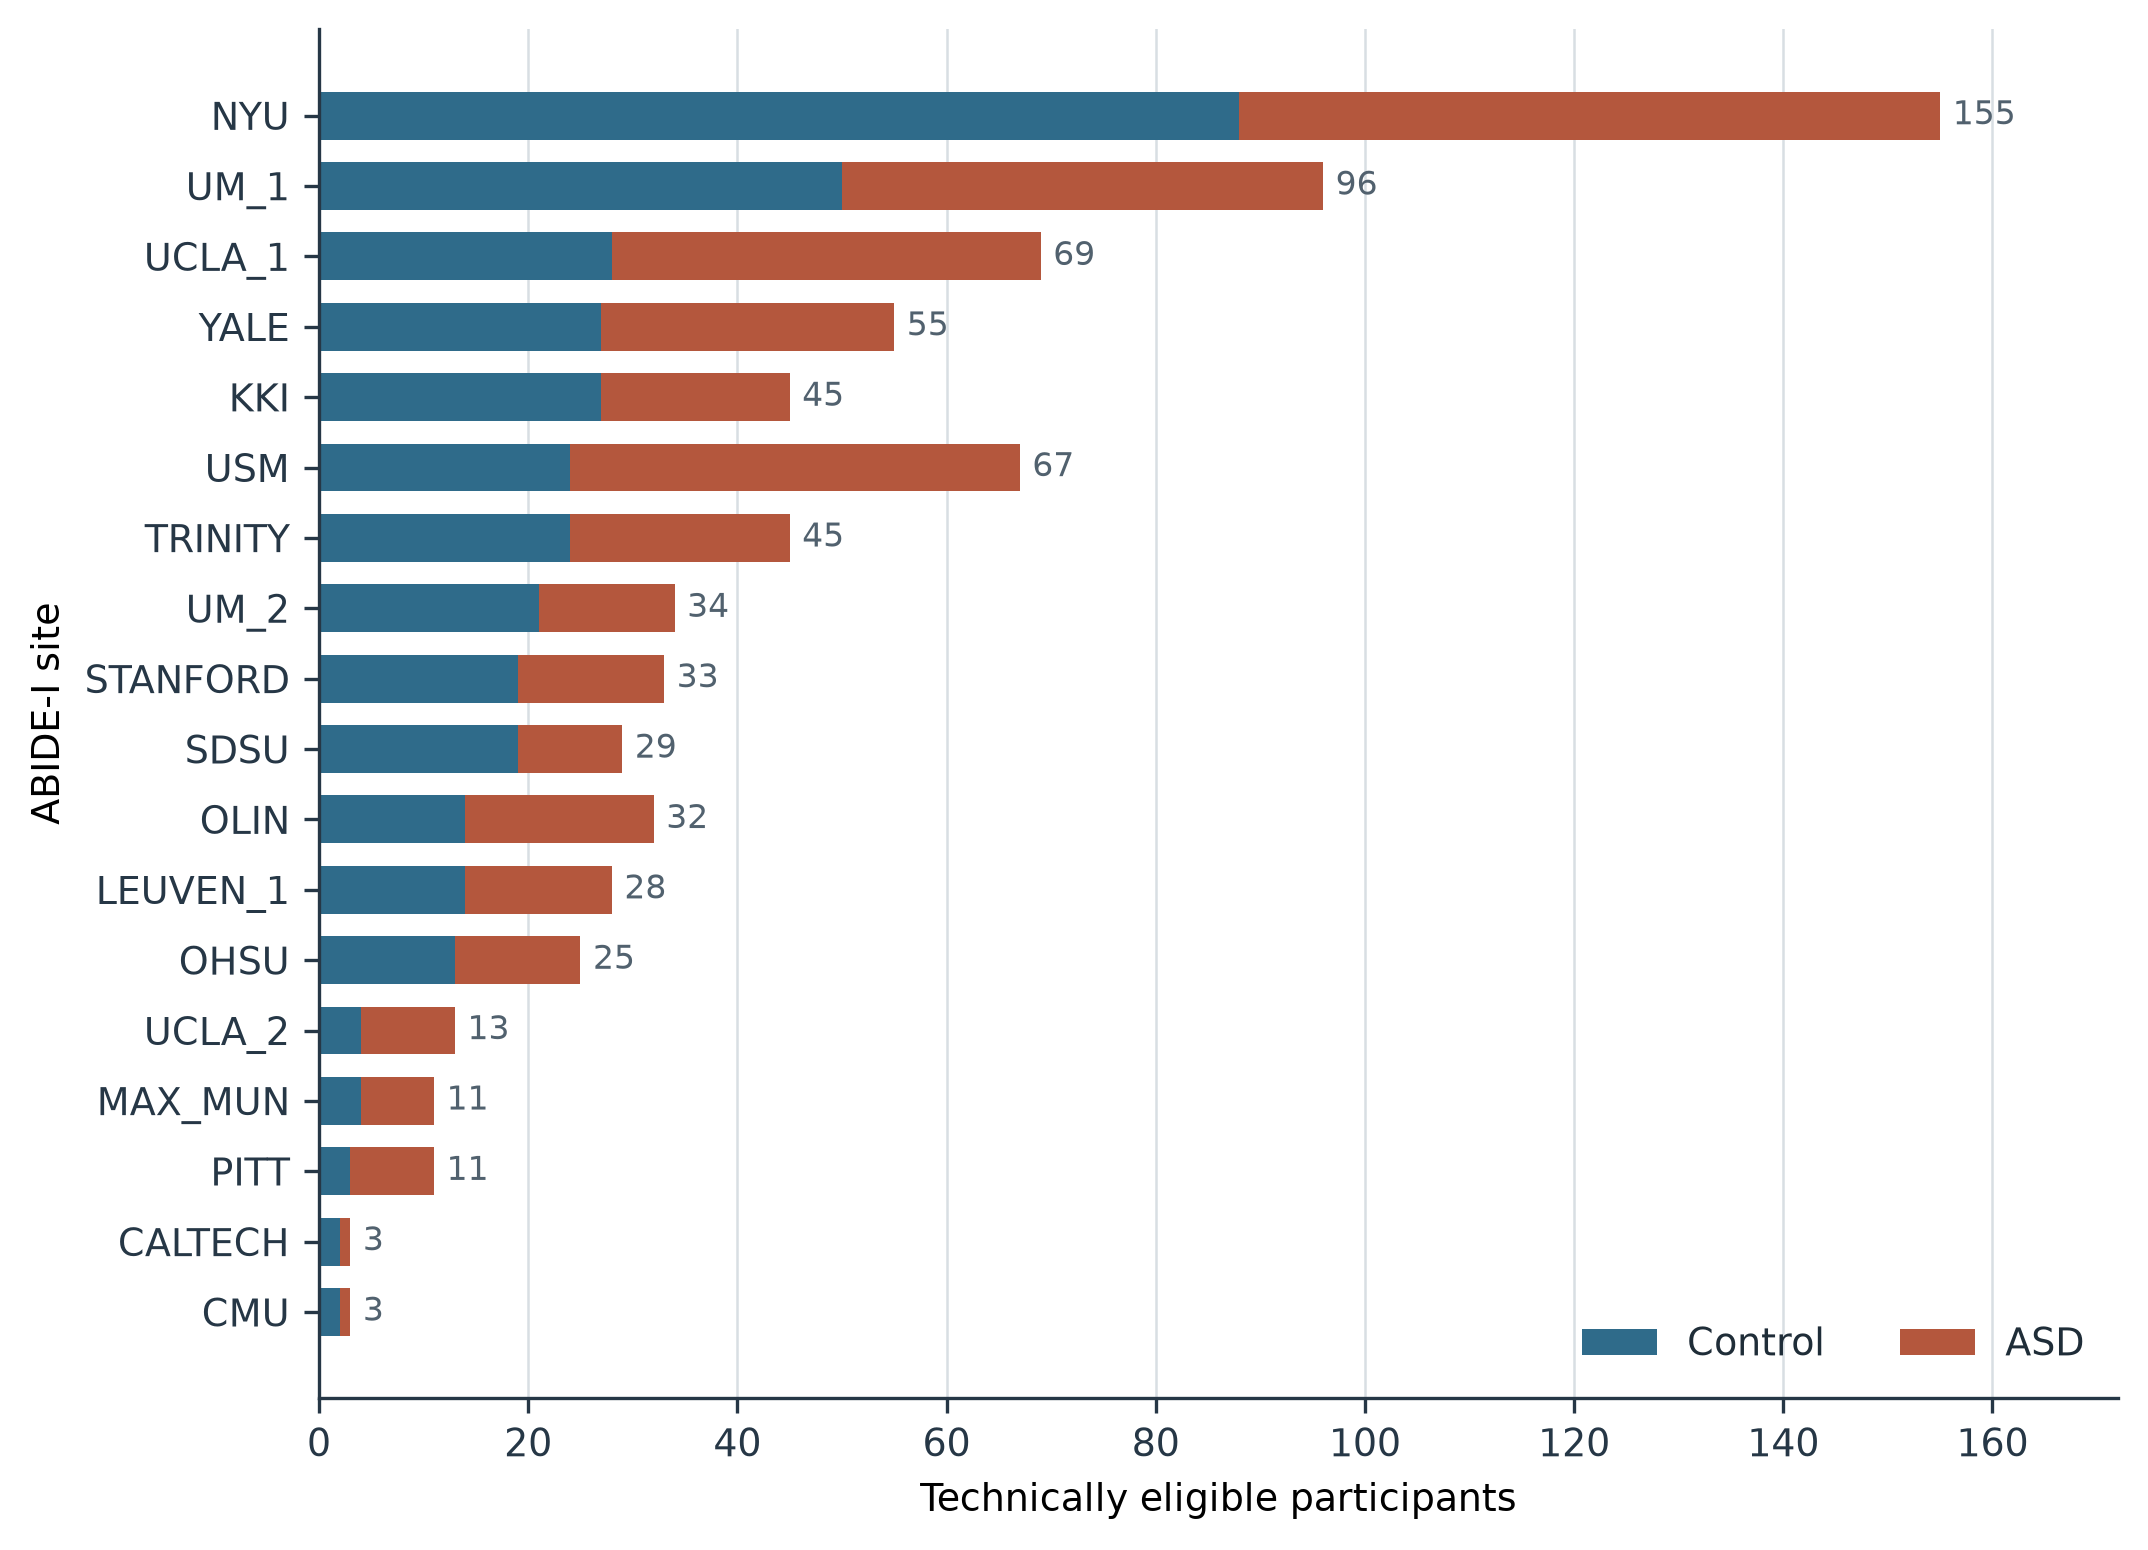
\includegraphics[width=0.88\textwidth]{site_composition.png}
  \caption{Participant composition of the frozen technically eligible cohort.
  Sites varied in both total size and class balance, motivating site-level
  evaluation and equal-site aggregation. This is a descriptive count figure,
  not a performance result.}
  \label{fig:site-composition}
\end{figure}

Technical eligibility does not imply population representativeness. Site
composition remained heterogeneous, as shown in \cref{fig:site-composition}.
That variation is handled in evaluation and uncertainty estimation rather
than erased from the data.

\subsection{Connectome construction}

For each participant, Pearson correlations were computed between every pair
of ROI time series and transformed with Fisher's $r$-to-$z$ function. The
diagonal was set to zero. The resulting matrix was finite and symmetric. Its
6,670 lower-triangle entries formed the feature vector for classical models.
For neural models, each node received its full 116-value connectivity row.

\begin{figure}[htbp]
  \centering
  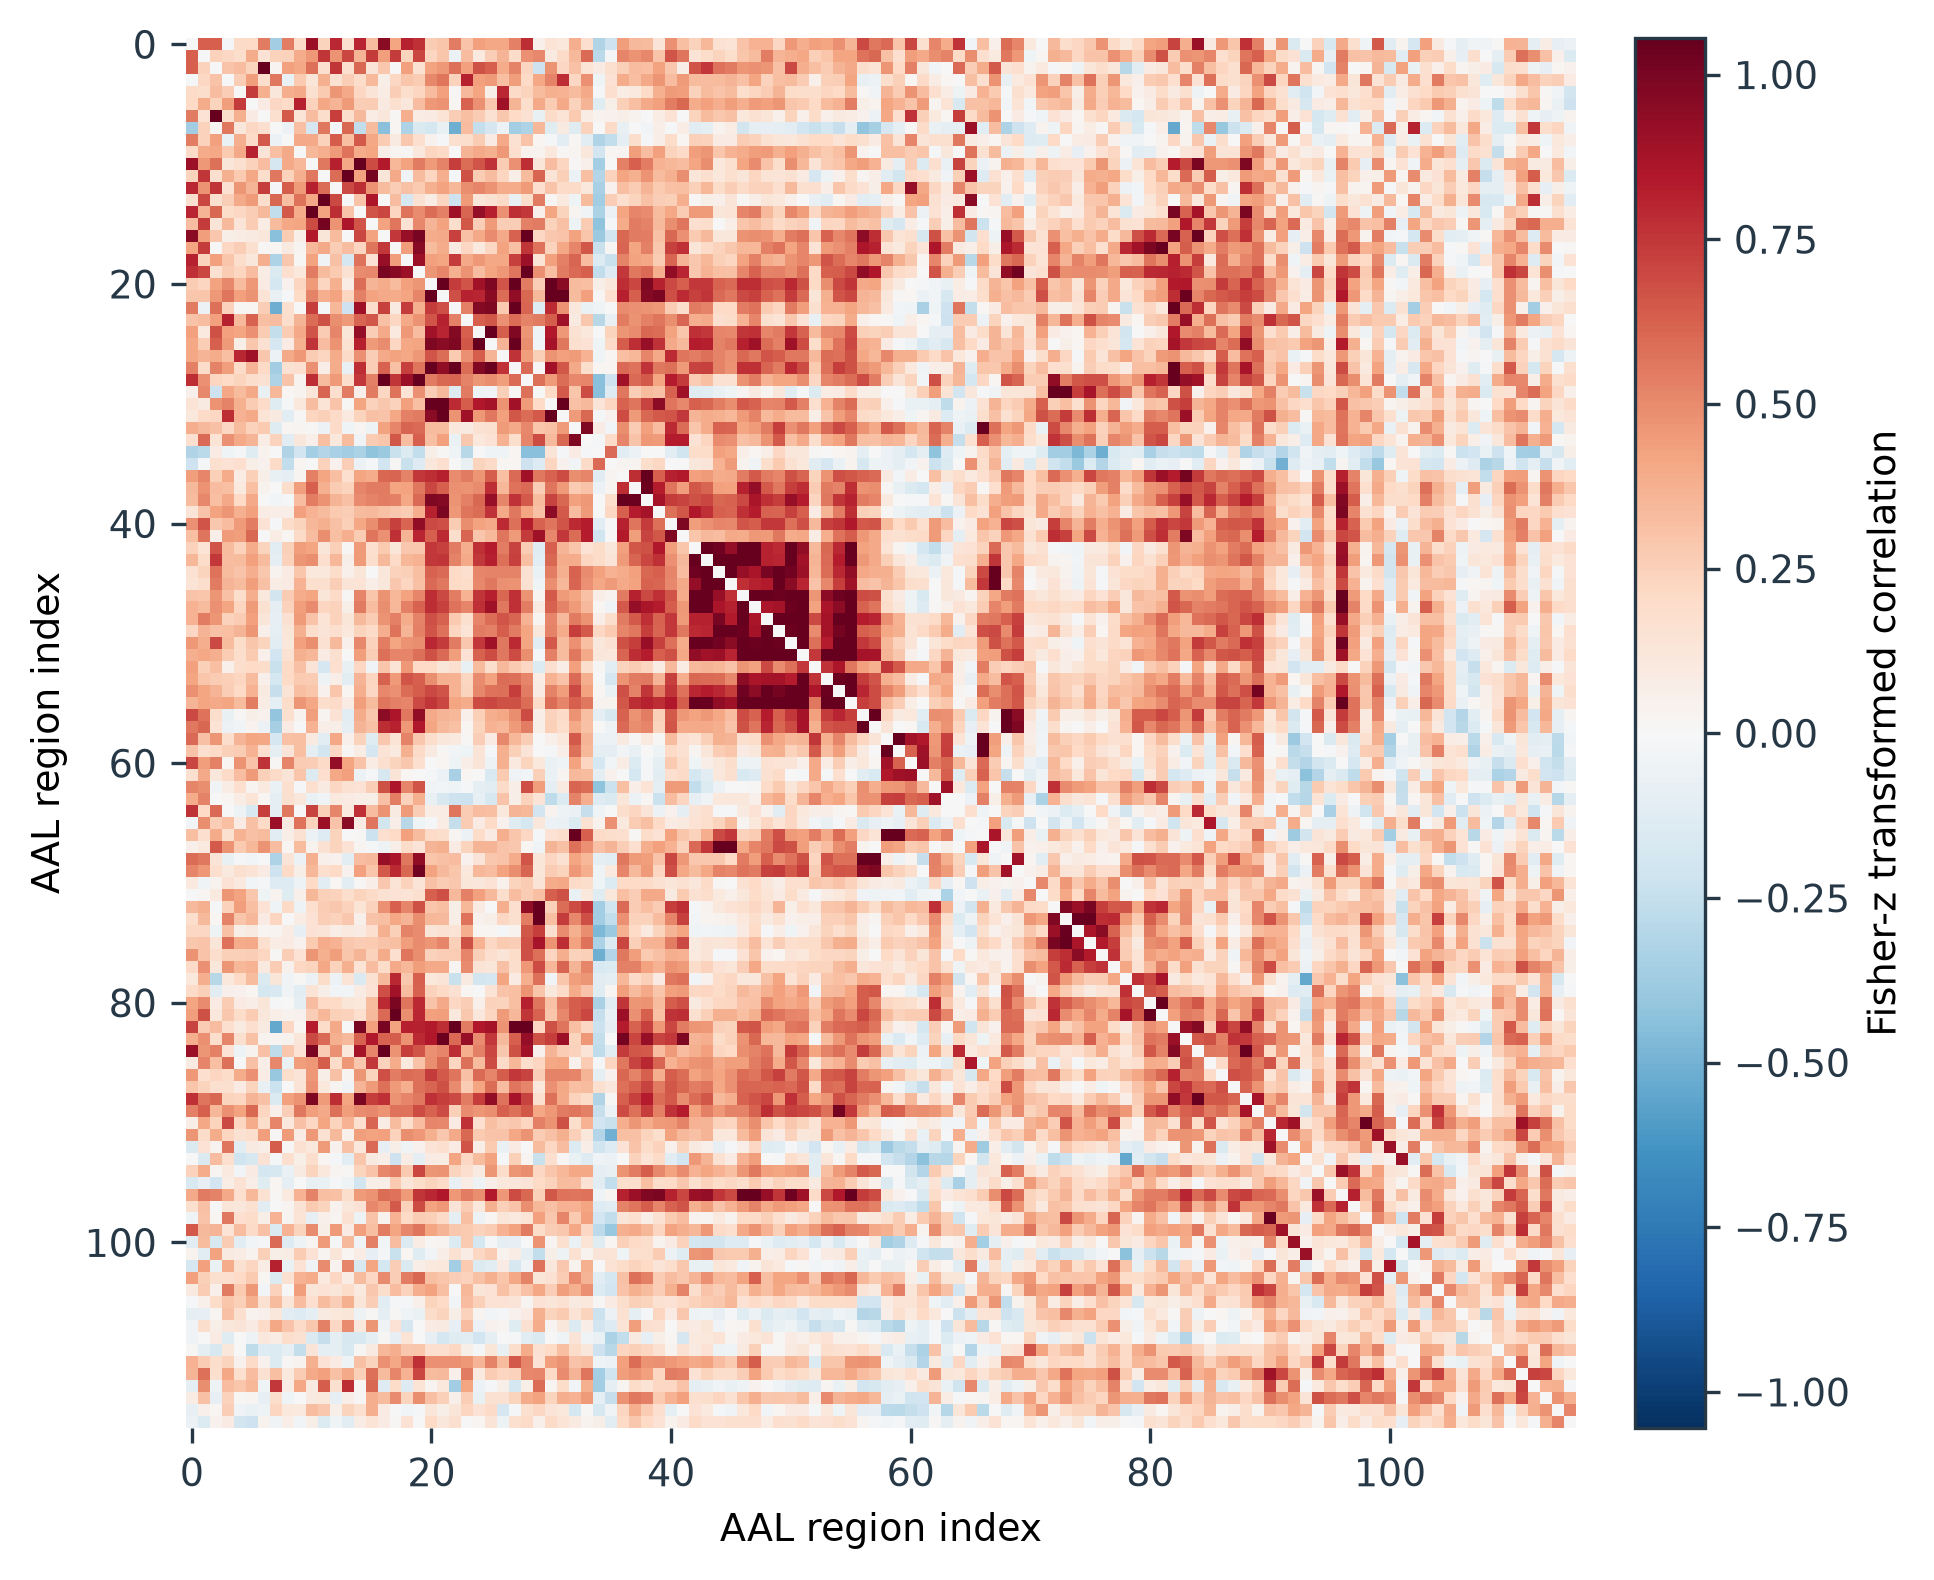
\includegraphics[width=0.71\textwidth]{example_connectome.png}
  \caption{A deterministic example from the frozen archive illustrating a
  participant-level Fisher-$z$ functional-connectivity matrix. Red and blue
  indicate positive and negative statistical associations. They are not
  interpreted as excitation, inhibition, anatomy, or causal flow.}
  \label{fig:connectome}
\end{figure}

At nonzero density, graphs retained the strongest positive off-diagonal
associations symmetrically at 1, 5, 10, and 20 percent. Density zero supplied
the matched identity or learned-local anchor. Negative associations remained
part of the node connectivity profiles but were not used as propagation edges.
This was a pre-specified computational choice, not a biological claim.

\subsection{Classical baselines}

Three logistic models provided practical references. The first used age, sex,
mean framewise displacement, and usable scan length. The second used all
vectorized connectome features with elastic-net regularization, which combines
$\ell_1$ and $\ell_2$ penalties for correlated high-dimensional predictors
\cite{zou2005elastic}. The third combined connectome features and covariates.
All scaling, feature processing, and tuning were fitted on training sites only.

\subsection{Shared neural backbone and operator controls}

The neural variants shared the encoder, hidden width, two propagation layers,
nonlinearities, normalization, dropout, pooling, classifier, optimizer,
training schedule, and tuning budget. The controlled difference was the
propagation rule or the map capacity needed to isolate it.

\begin{table}[htbp]
\centering
\caption{Neural operator and capacity controls.}
\label{tab:operators}
\begin{tabularx}{\textwidth}{@{}p{2.8cm}Y Y@{}}
\toprule
\textbf{Variant} & \textbf{Operation} & \textbf{Purpose} \\
\midrule
Identity & No inter-node propagation & Tests whether message passing adds value. \\
Learned-local & Learns the BuNN node-wise maps but does not diffuse between nodes & Separates map-generator capacity from transport. \\
GCN & Normalized neighborhood aggregation & Standard graph-diffusion reference. \\
Trivial bundle & Bundle diffusion with identity transport maps & Separates the diffusion construction from learned transport. \\
Learned BuNN & Learned orthogonal node maps followed by bundle diffusion & Tests the proposed transport operator. \\
\bottomrule
\end{tabularx}
\end{table}

\begin{figure}[htbp]
  \centering
  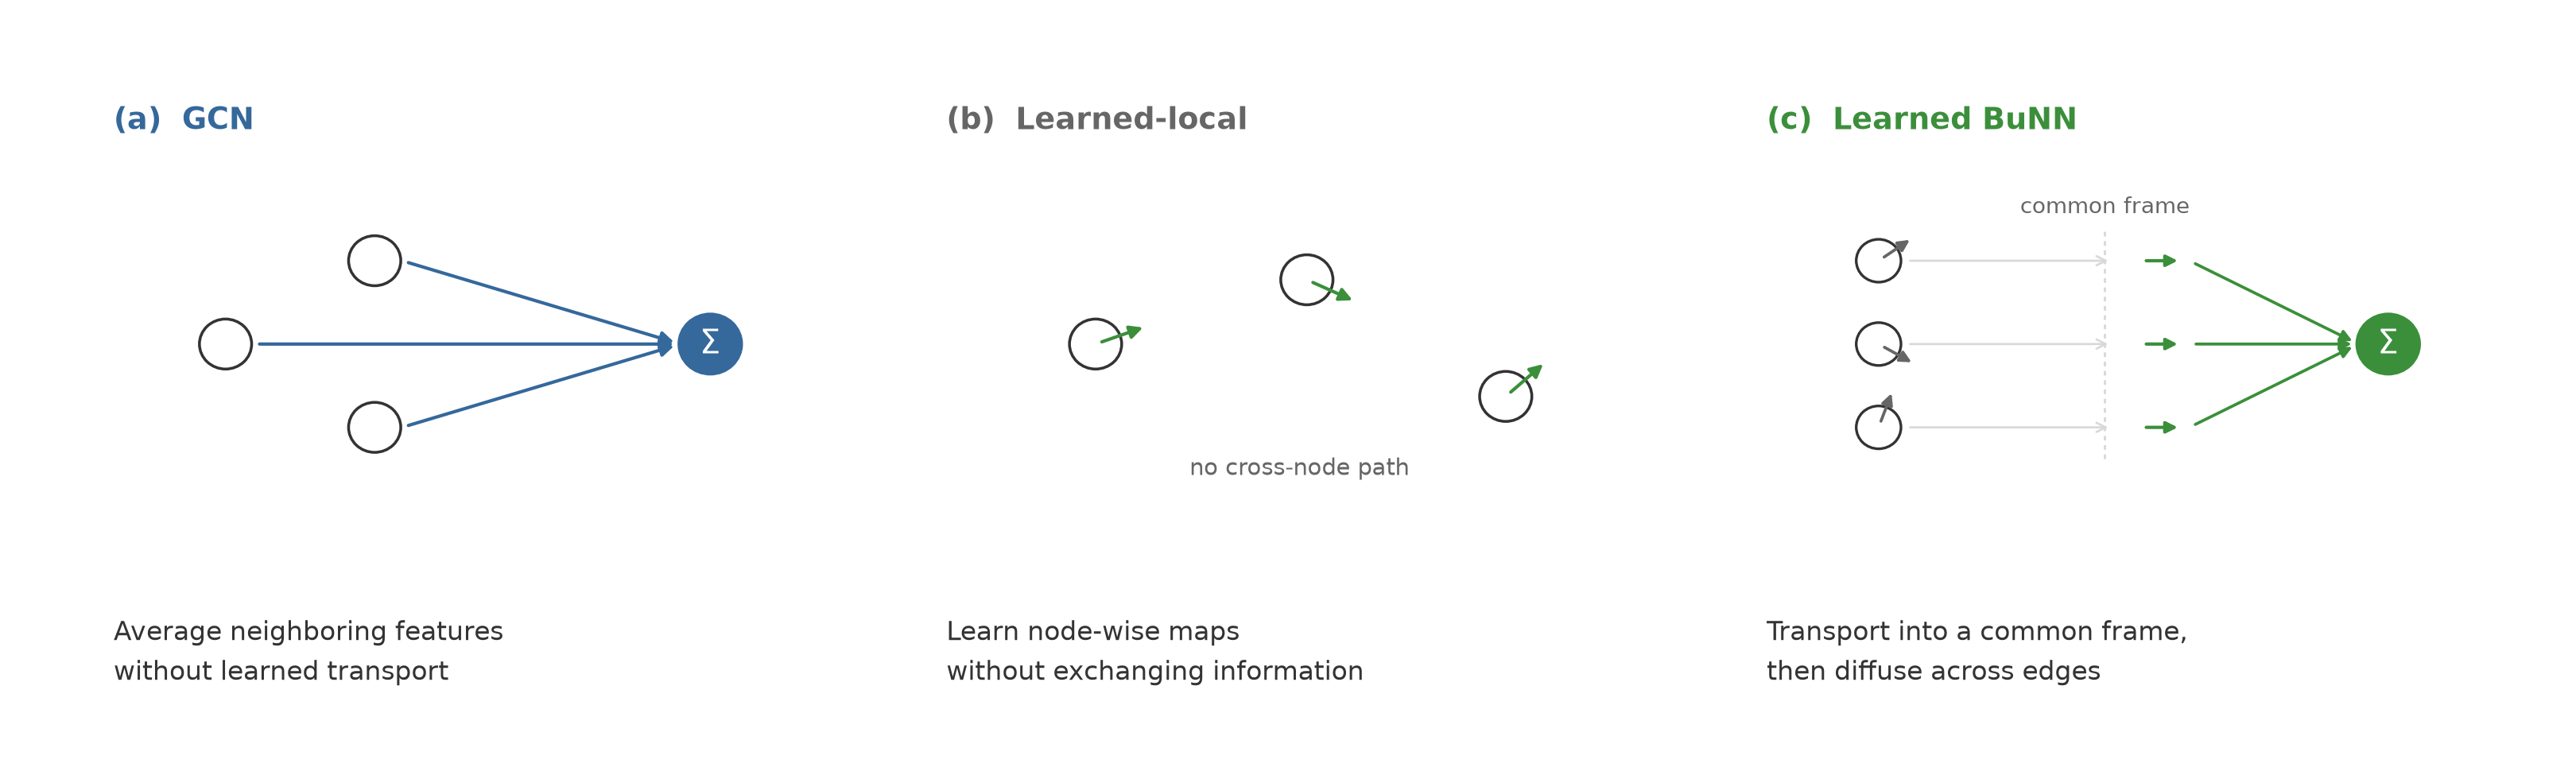
\includegraphics[width=0.98\textwidth]{operator_schematic.png}
  \caption{Computational distinction among GCN aggregation, the learned-local
  capacity control, and learned bundle transport. The schematic does not
  represent biological signal flow.}
  \label{fig:operator}
\end{figure}

\subsection{Nested held-out-site evaluation}

Each site served once as the outer test site. Four grouped folds within the
remaining sites selected among four equal-budget AdamW candidates using two
tuning seeds. The selected configuration was refitted with five fixed final
seeds. Test-site data did not enter scaling, tuning, stopping, or model
selection. The primary predictive endpoint was the unweighted mean of
held-out-site balanced accuracies. This gives each acquisition site equal
influence. Pooled balanced accuracy and AUROC were secondary.

\subsection{Density-curve and representation estimands}

The primary predictive estimand was the normalized trapezoidal area under the
balanced-accuracy curve across the full density grid. GCN and trivial-bundle
curves used identity at zero density. The learned-BuNN curve used the
parameter-matched learned-local anchor. Comparing the whole curve avoided
choosing a favorable density after viewing the results.

After each propagation layer, BuNN embeddings were transported into a common
learned frame before node comparisons. Normalized effective rank at layer 2
was the primary representation endpoint. Secondary measures included
normalized dispersion, mean pairwise cosine similarity, invariant
edge-transport distance, and encoder-to-layer-2 rank change. These measures
describe co-occurring representation behavior. They do not prove that a
representation change caused a prediction change.

\subsection{Statistical analysis and decision rule}

The five final seeds were averaged within each site and configuration before
site-level inference. Confidence intervals used 10,000 paired bootstrap
resamples of the 18 held-out sites. Curve contrasts also received exact
two-sided paired sign-flip tests. Density-specific tests were secondary and
Holm-corrected within each named family.

A positive architectural result required all three of the following:
\begin{enumerate}
  \item stronger common-frame representation preservation than GCN;
  \item better held-out prediction than GCN and the matched no-propagation
  controls; and
  \item performance above the strongest regularized non-graph baseline.
\end{enumerate}

A confidence interval containing zero was reported as no detected advantage.
A practically meaningful gain was ruled out only if the upper confidence
bound fell below the pre-specified 0.03 balanced-accuracy margin.

\subsection{Run integrity and reproducibility}

Long-running jobs wrote atomic per-site checkpoints and recorded immutable
hashes for data, configuration, and source code. Site ownership, restart
validation, canonical merging, and independent completion audits protected
the parallel run. The neural artifact was checked for coverage, recomputed
metrics, diagnostics, runtime records, and warnings before unblinding. Values
in the report are generated from a hash-bound result snapshot rather than
copied manually.

\subsection{Post-hoc accepted-checkpoint intervention audit}

After Study 1 was frozen, a separate protocol tested what the 360 accepted
learned-BuNN checkpoints depended on without refitting them. Each checkpoint
was first required to reproduce its archived held-out probabilities within
$10^{-6}$. Four scientific interventions were then compared with unaltered
inference: replacing learned maps with identity maps, shuffling learned maps
between nodes, replacing them with random orthogonal maps, and rewiring each
participant graph by double-edge swaps that preserved its exact degree
sequence. An encoded-node permutation served only as an equivariance check.

The randomized families used 100 stored randomizations, shared across the
five model seeds. Balanced accuracy was calculated for each seed and
randomization, randomizations were averaged within the site-density cell,
and seeds were then averaged. The four density-specific paired effects were
averaged within site, followed by an unweighted mean over the 18 sites. The
effect direction was always intervention minus unaltered BuNN. Uncertainty
used 10,000 paired site-bootstrap samples. Two-sided exact sign-flip tests
enumerated all $2^{18}$ site sign assignments, with Holm correction across
the four primary interventions.

Secondary endpoints were absolute probability change, classification flips,
AUROC, sensitivity, specificity, and changes in the four final-layer
gauge-aware diagnostics. Associations between representation and prediction
changes were descriptive Spearman correlations across the 72 site-density
cells, not mediation tests. The complete run was archived and audited before
the analysis protocol and code were frozen. The analyzer passed synthetic
known-answer tests before a single acknowledged unblinding invocation, and
an independent recomputation audit passed before interpretation.

\section{Results}

\subsection{Classical baseline performance}

The connectome elastic net was the strongest classical model, with equal-site
balanced accuracy 0.6401. Adding covariates produced 0.6336, while covariates
alone produced 0.5652. Imaging features therefore carried cross-site
predictive information under this pipeline, but the result is computational
and should not be described as clinical diagnostic performance.

\begin{table}[htbp]
\centering
\caption{Held-out-site performance of the classical baselines.}
\label{tab:baselines}
\begin{tabularx}{\textwidth}{@{}Y r r r@{}}
\toprule
\textbf{Model} & \textbf{Equal-site BA} & \textbf{Pooled BA} & \textbf{Pooled AUROC} \\
\midrule
Covariates-only logistic regression & 0.5652 & 0.5629 & 0.5973 \\
Connectome elastic net & \textbf{0.6401} & \textbf{0.6495} & \textbf{0.6794} \\
Connectome + covariates elastic net & 0.6336 & 0.6428 & 0.6773 \\
\bottomrule
\end{tabularx}
\end{table}

\subsection{Predictive performance across graph density}

All diffusion curves declined as graph density increased
(\cref{fig:predictive}). The learned-BuNN minus GCN normalized curve-area
difference was \BunnGcnEstimate{} (95\% confidence interval
[\BunnGcnCILow{}, \BunnGcnCIHigh{}]; exact $p=\BunnGcnP$). The interval crossed
zero, so no predictive advantage was detected. Its upper bound was also below
the pre-specified 0.03 margin. This rules out a gain of that size for the
specified estimand and pipeline, but not every smaller effect or every other
BuNN design.

\begin{figure}[htbp]
  \centering
  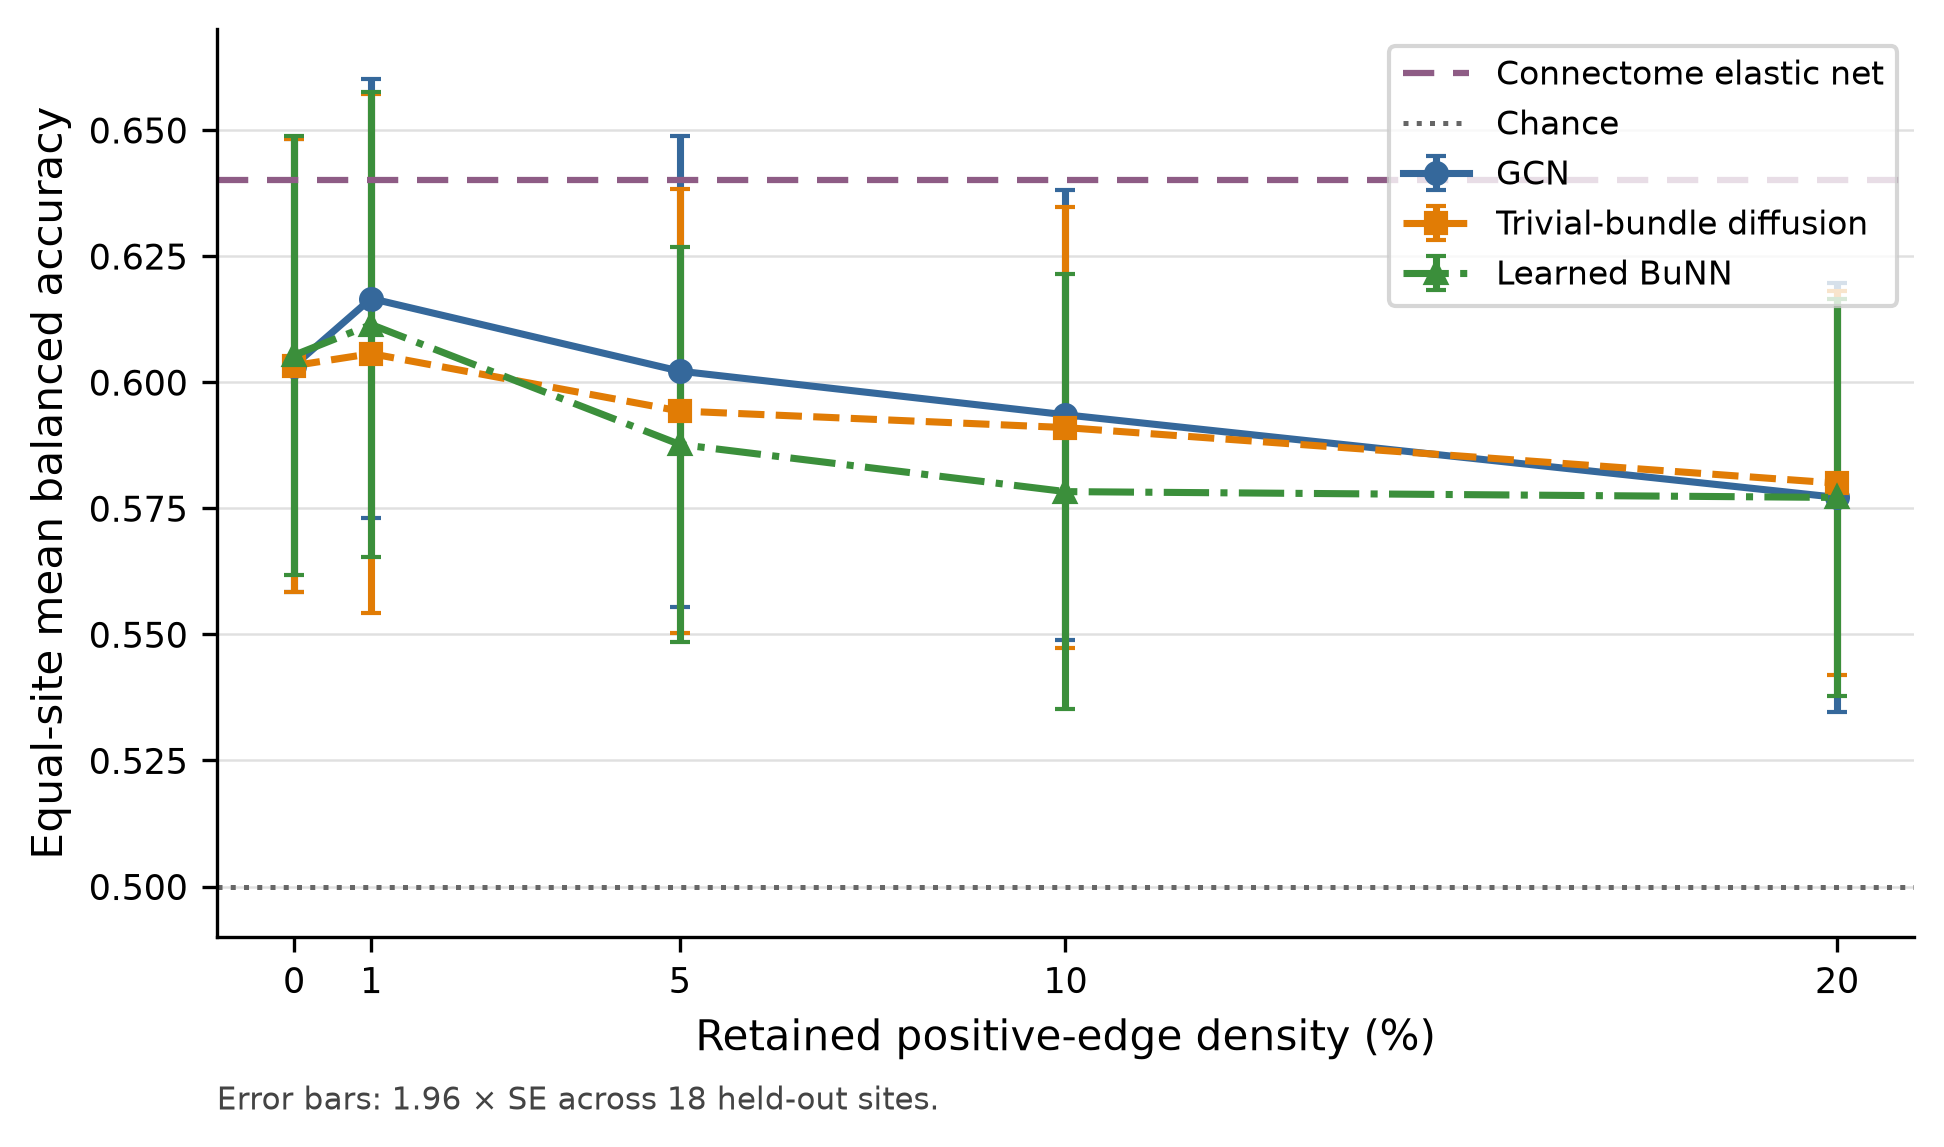
\includegraphics[width=0.98\textwidth]{predictive_density_curves.png}
  \caption{Equal-site mean held-out balanced accuracy across the pre-specified
  positive-edge density grid. Error bars show 1.96 standard errors across
  sites for visualization. Confirmatory inference used paired site bootstrap
  and exact sign-flip tests on the locked curve estimand.}
  \label{fig:predictive}
\end{figure}

Against the site-matched connectome elastic net, the learned-BuNN curve
difference was \BunnElasticEstimate{} (95\% confidence interval
[\BunnElasticCILow{}, \BunnElasticCIHigh{}]; exact $p=\BunnElasticP$). The
interval lay entirely below zero. Comparisons with identity and learned-local
controls also failed the positive-result rule.

\begin{table}[htbp]
\centering
\caption{Pre-specified predictive contrasts. Estimates are balanced-accuracy differences.}
\label{tab:confirmatory}
\small
\begin{tabularx}{\textwidth}{@{}Y r r r@{}}
\toprule
\textbf{Contrast} & \textbf{Estimate} & \textbf{95\% CI} & \textbf{Exact $p$} \\
\midrule
BuNN curve $-$ GCN curve & $-0.0096$ & $[-0.0366,\ 0.0115]$ & 0.524 \\
BuNN curve $-$ trivial-bundle curve & $-0.0062$ & $[-0.0293,\ 0.0108]$ & 0.681 \\
BuNN nonzero mean $-$ learned-local & $-0.0167$ & $[-0.0347,\ 0.0009]$ & 0.096 \\
BuNN nonzero mean $-$ identity & $-0.0146$ & $[-0.0320,\ 0.0018]$ & 0.116 \\
BuNN curve $-$ connectome elastic net & $-0.0552$ & $[-0.0830,\ -0.0275]$ & 0.0018 \\
\bottomrule
\end{tabularx}
\end{table}

\subsection{Common-frame representation behavior}

The raw BuNN effective-rank curve appeared higher than the GCN curve, but its
learned-local zero-density anchor was already high. After subtracting each
operator's matched anchor, the normalized effective-rank contrast was
\RankEstimate{} (95\% confidence interval [\RankCILow{}, \RankCIHigh{}]). Its
direction was opposite to the proposed BuNN preservation advantage.
Normalized dispersion and pairwise cosine similarity showed the same broad
pattern.

\begin{figure}[htbp]
  \centering
  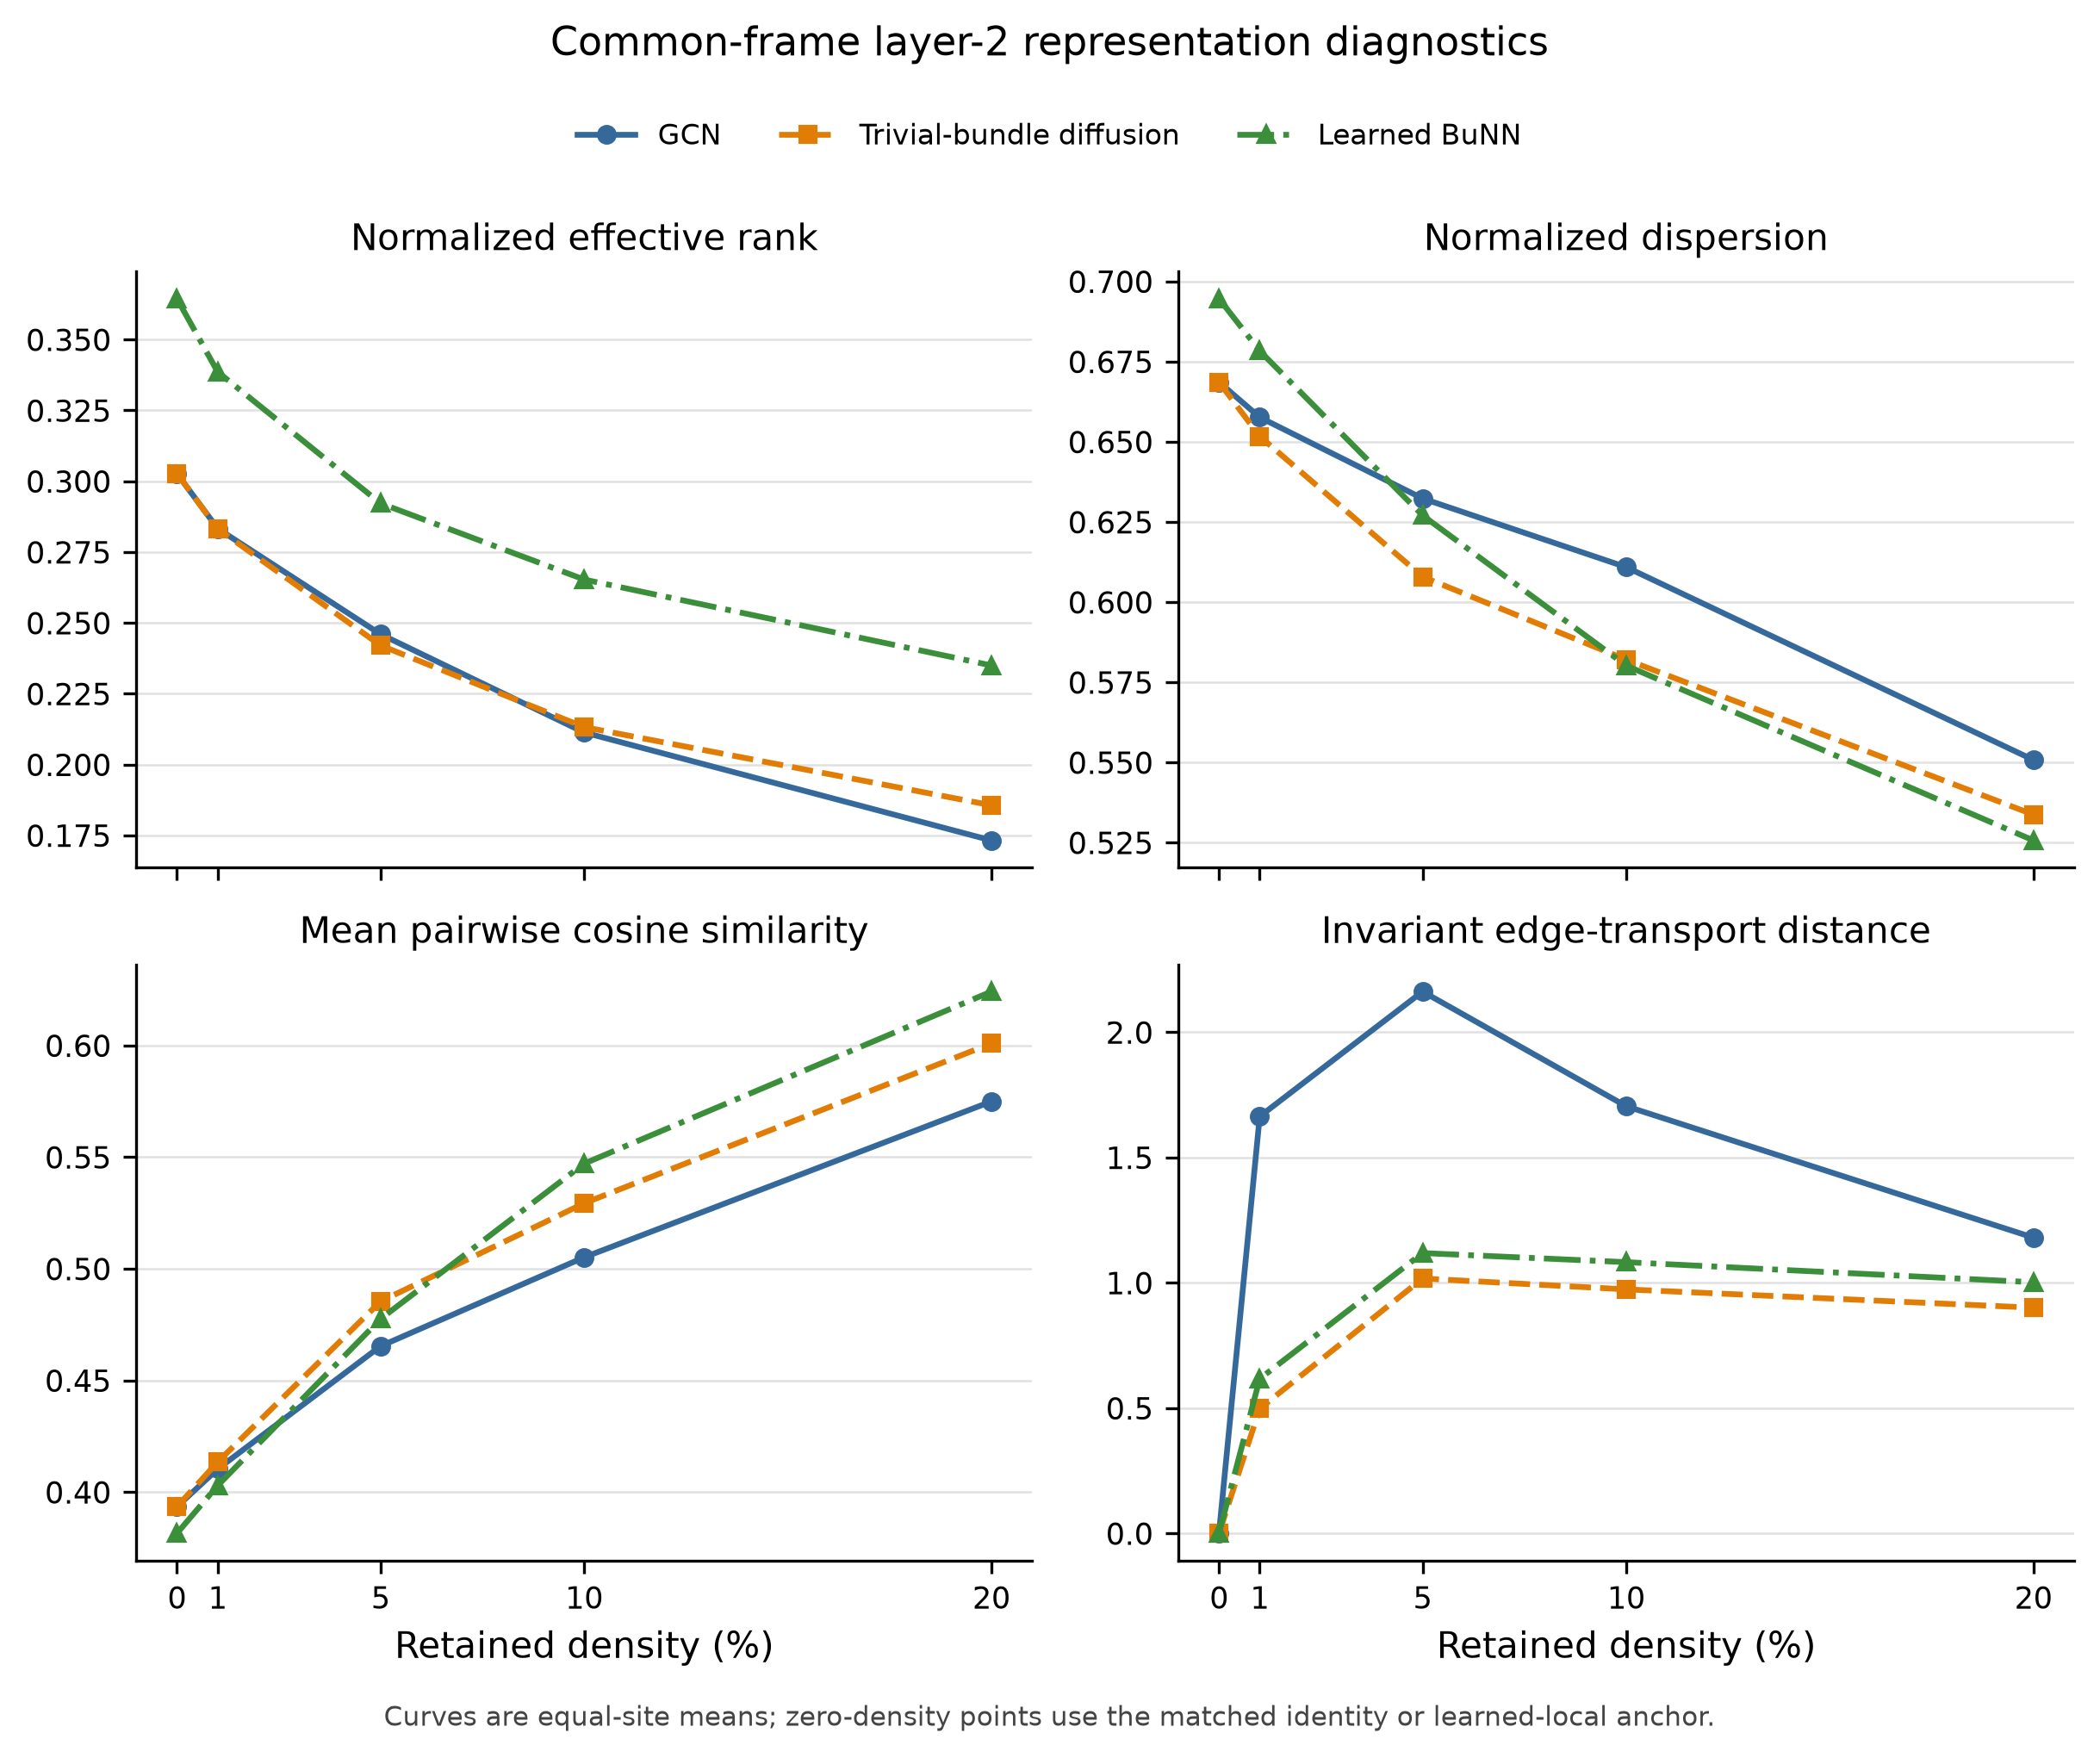
\includegraphics[width=0.98\textwidth]{representation_density_curves.png}
  \caption{Equal-site common-frame representation diagnostics at layer 2.
  Zero-density points use the matched identity or learned-local anchor. Raw,
  unaligned BuNN node embeddings were not compared.}
  \label{fig:representation}
\end{figure}

The learned-local control is decisive for interpretation. Without it, extra
map-generator capacity could be mistaken for information preserved by
inter-node transport. The matched result gives no support for that transport
explanation. These diagnostics remain computational measurements and do not
identify a biological mechanism.

\begin{table}[htbp]
\centering
\caption{BuNN-minus-GCN matched-anchor representation contrasts.}
\label{tab:representation}
\small
\begin{tabularx}{\textwidth}{@{}Y r r@{}}
\toprule
\textbf{Layer-2 endpoint} & \textbf{Estimate} & \textbf{95\% CI} \\
\midrule
Normalized effective rank (primary) & $-0.0072$ & $[-0.0131,\ -0.0010]$ \\
Normalized dispersion & $-0.0417$ & $[-0.0523,\ -0.0306]$ \\
Mean pairwise cosine similarity & $0.0415$ & $[0.0319,\ 0.0507]$ \\
Invariant edge-transport distance & $-0.6436$ & $[-0.8205,\ -0.4720]$ \\
Encoder-to-layer-2 effective-rank change & $-0.0056$ & $[-0.0144,\ 0.0048]$ \\
\bottomrule
\end{tabularx}
\end{table}

\subsection{Accepted-checkpoint mechanism audit}

The post-hoc intervention audit showed that the learned maps were not dormant
components. Replacing them with random orthogonal maps reduced held-out
balanced accuracy by 8.86 percentage points (95\% paired site-bootstrap
interval $[-12.36,-4.78]$; exact sign-flip $p=0.00095$;
Holm-adjusted $p=0.0038$). The effect was negative at every density and in 15
of 18 sites after averaging densities. This was the only intervention that
passed the pre-specified four-contrast multiplicity-controlled test.

Identity maps produced a 4.72-point reduction (95\% interval
$[-8.56,-0.29]$). Its unadjusted exact $p$ was 0.0468, but its adjusted
$p$ was 0.1404. Shuffling learned maps between nodes caused a smaller
1.94-point reduction (95\% interval $[-3.77,0.05]$; adjusted
$p=0.1404$). Degree-preserving rewiring caused a 1.23-point reduction
(95\% interval $[-2.49,-0.05]$; adjusted $p=0.1404$). Bootstrap intervals
and sign-flip tests answer related but different questions; the adjusted
sign-flip result controls the four named primary tests.

\begin{table}[htbp]
\centering
\caption{Accepted-checkpoint intervention effects. Estimates are intervened
minus unaltered BuNN balanced accuracy in percentage points.}
\label{tab:e1-primary}
\small
\begin{tabularx}{\textwidth}{@{}Y r r r@{}}
\toprule
\textbf{Intervention} & \textbf{Estimate} & \textbf{95\% CI} & \textbf{Holm $p$} \\
\midrule
Identity maps & $-4.72$ & $[-8.56,-0.29]$ & 0.1404 \\
Shuffled learned maps & $-1.94$ & $[-3.77,0.05]$ & 0.1404 \\
Random orthogonal maps & $-8.86$ & $[-12.36,-4.78]$ & \textbf{0.0038} \\
Degree-preserving rewiring & $-1.23$ & $[-2.49,-0.05]$ & 0.1404 \\
\bottomrule
\end{tabularx}
\end{table}

\begin{figure}[htbp]
  \centering
  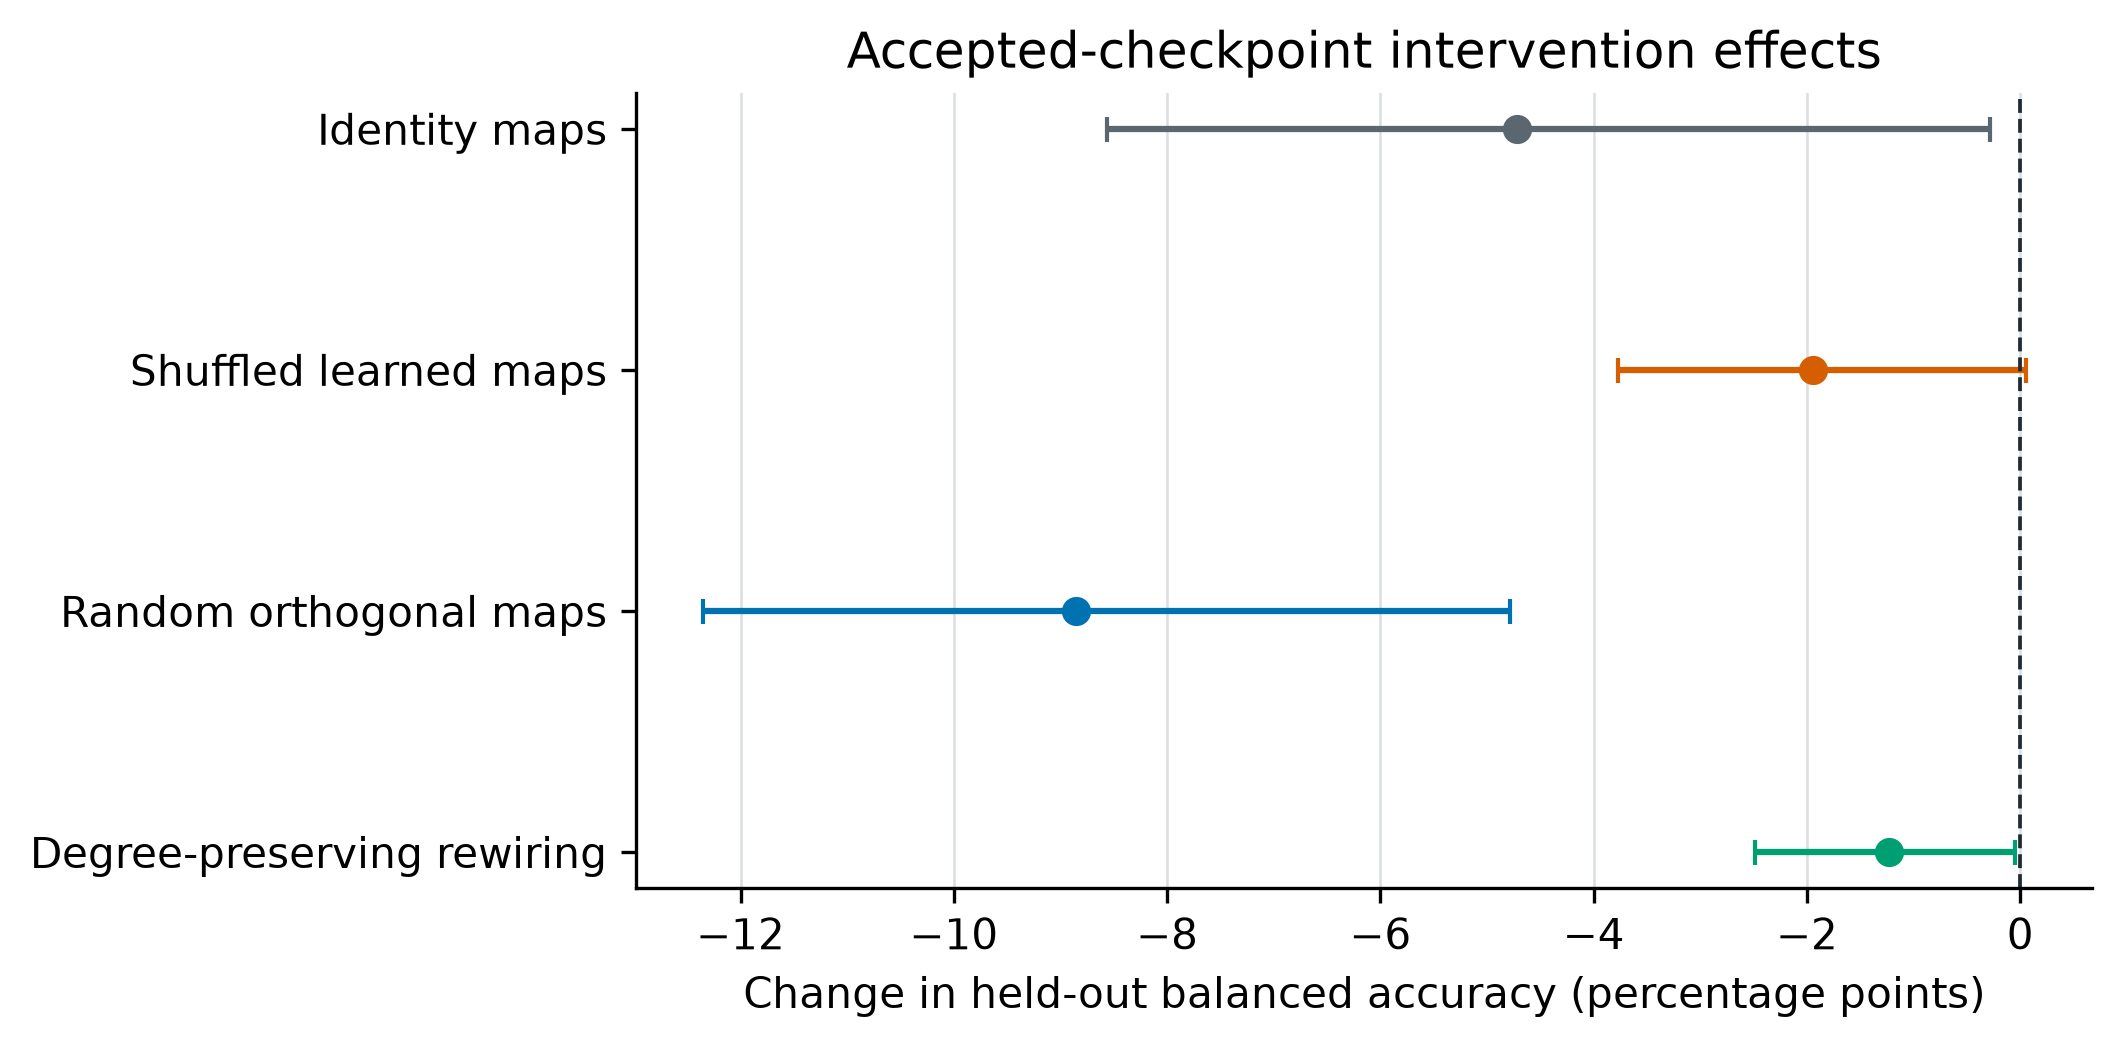
\includegraphics[width=0.98\textwidth]{e1_primary_intervention_forest.png}
  \caption{Overall E1 intervention effects with 95\% paired site-bootstrap
  intervals. Negative values mean that disrupting the component reduced the
  accepted checkpoint's held-out balanced accuracy. Statistical decisions
  use the Holm-adjusted exact sign-flip tests in \cref{tab:e1-primary}.}
  \label{fig:e1-primary}
\end{figure}

The random-map effect remained negative at 1, 5, 10, and 20 percent density
(\cref{fig:e1-density}). Identity maps had their largest effect at 1 percent
density. Shuffling maps and rewiring topology produced smaller effects that
often had density-specific intervals crossing zero. The density pattern
therefore does not look like a benefit confined to one hand-picked threshold.

\begin{figure}[htbp]
  \centering
  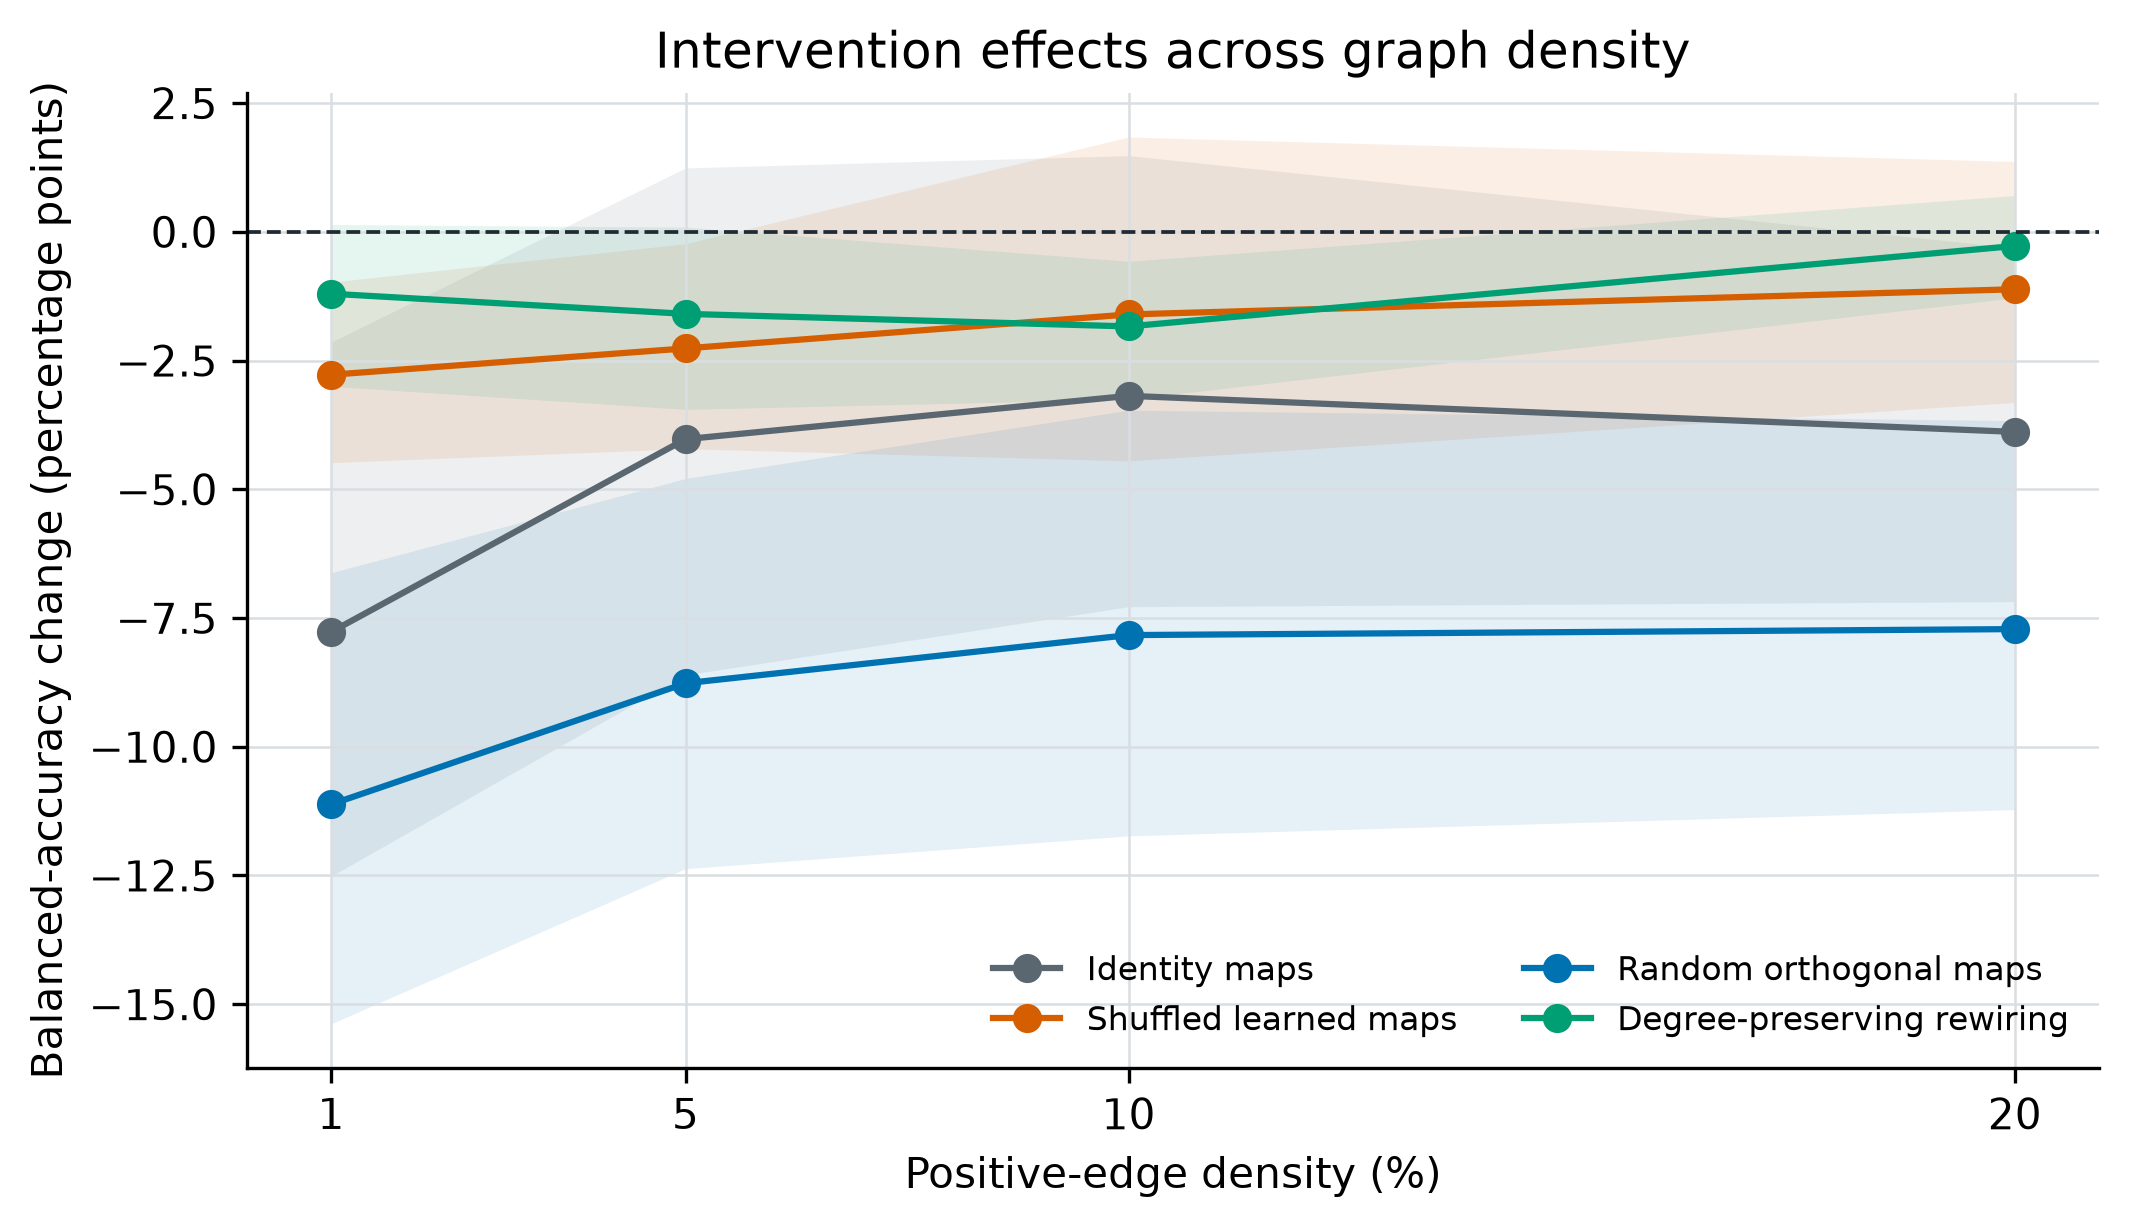
\includegraphics[width=0.98\textwidth]{e1_density_intervention_effects.png}
  \caption{Density-specific accepted-checkpoint intervention effects. Shaded
  regions are 95\% paired site-bootstrap intervals. These density-specific
  estimates are descriptive; the primary inference averages the four effects
  within site before equal-site analysis.}
  \label{fig:e1-density}
\end{figure}

The prediction changes were also practically visible. Random maps changed
49.46\% of binary decisions and reduced AUROC by 14.59 points. Identity maps
changed 34.41\% of decisions and reduced AUROC by 9.50 points. Shuffled maps
changed 15.12\% of decisions, while topology rewiring changed 6.96\%.
Random maps strongly reduced sensitivity while increasing specificity,
indicating a shift toward control predictions rather than symmetric noise.

All four interventions changed at least some gauge-aware diagnostics, but
those changes did not track predictive effects closely. Across the 72
site-density cells, the absolute descriptive Spearman correlations between
diagnostic changes and balanced-accuracy changes were at most 0.21
(\cref{fig:e1-association}). The measured representation summaries therefore
do not provide a simple predictive mechanism or a causal mediation result.

\begin{figure}[htbp]
  \centering
  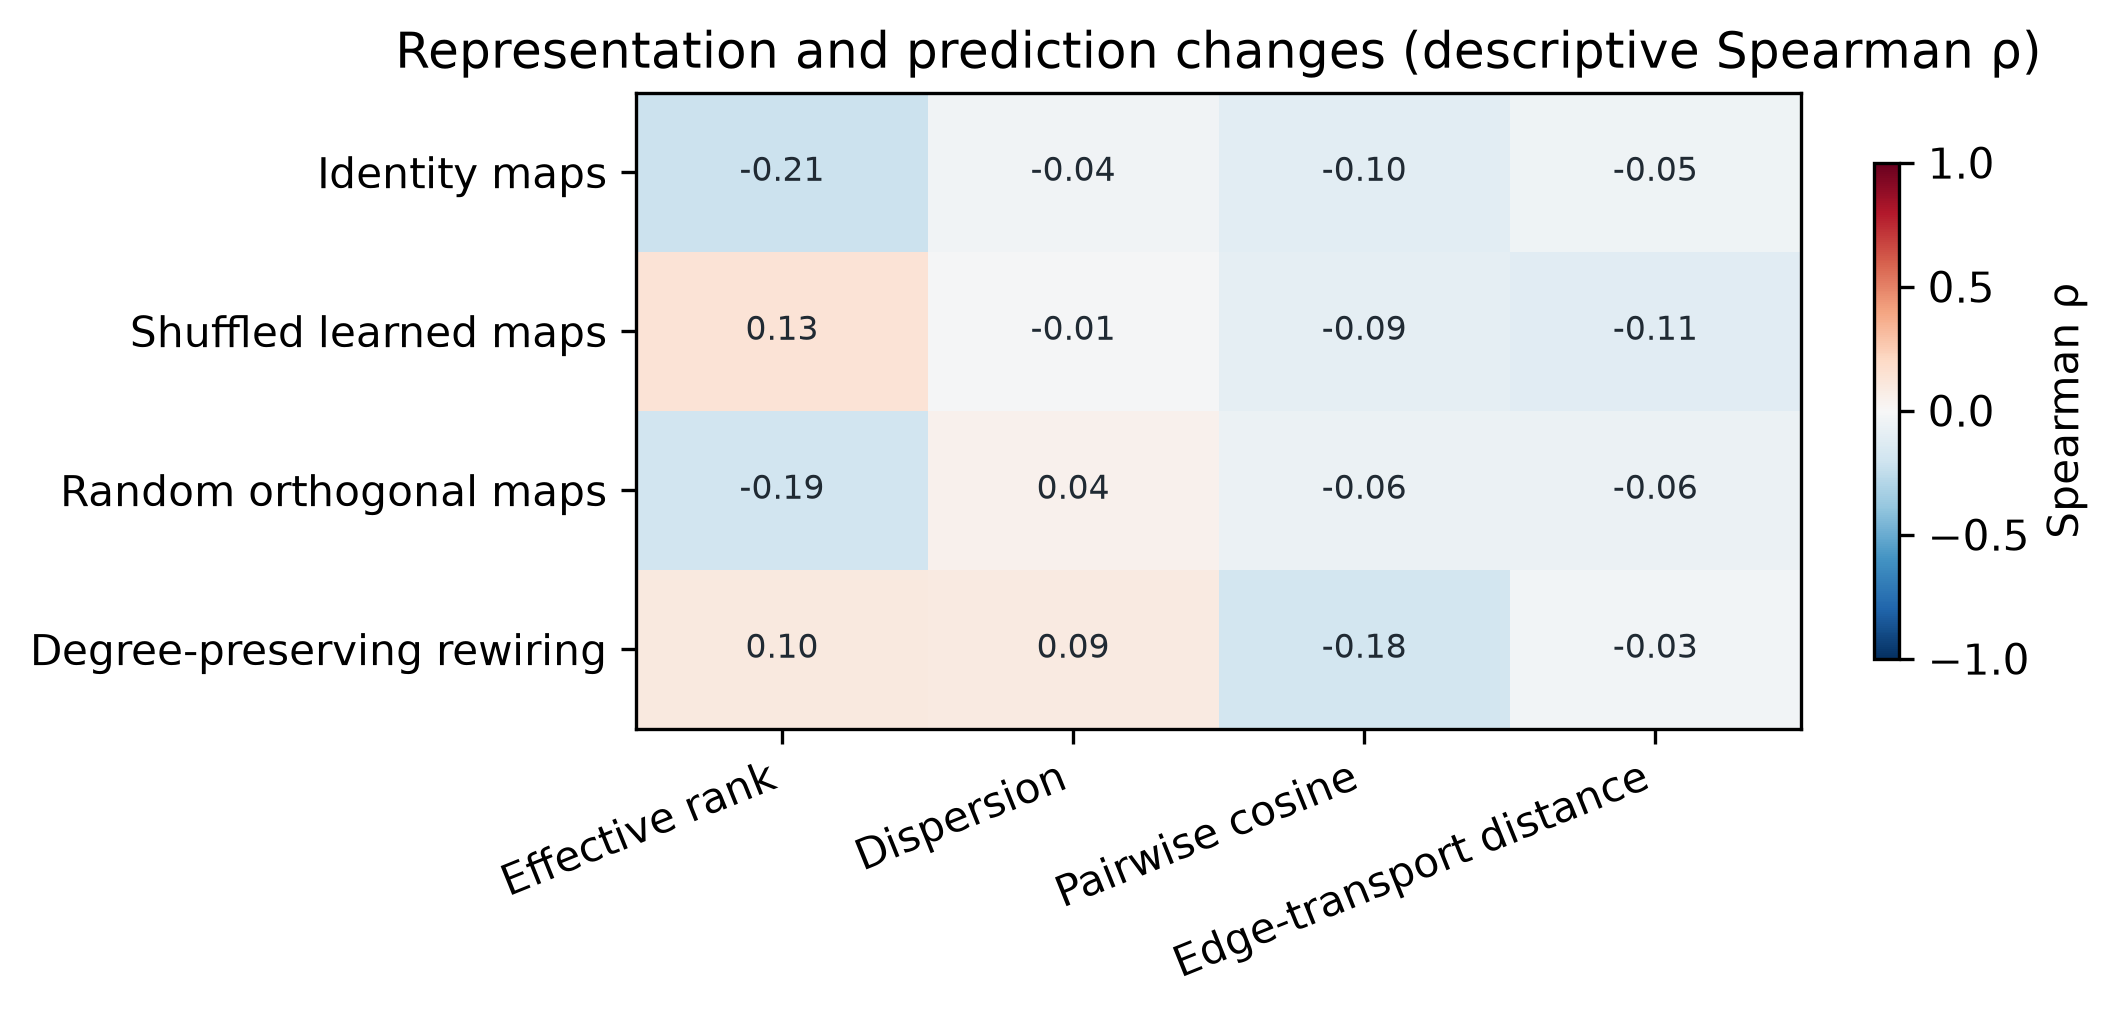
\includegraphics[width=0.98\textwidth]{e1_representation_prediction_associations.png}
  \caption{Descriptive association between final-layer gauge-aware diagnostic
  changes and balanced-accuracy changes across 72 site-density cells. The
  correlations are exploratory summaries, not multiplicity-controlled tests
  or evidence of causal mediation.}
  \label{fig:e1-association}
\end{figure}

\subsection{Site, seed, and weighting sensitivity}

Only \LeaveOneSitePositive{} of the \StudySites{} leave-one-site influence
estimates was positive, and no favorable exclusion interval lay above zero.
Two of five seed point estimates favored BuNN, but no favorable seed interval
excluded zero; one unfavorable interval lay below zero. Participant weighting
reversed the sign of the small BuNN--GCN point estimate, whereas the equal-site
mean and median remained negative. The pre-specified confirmatory estimand was
the equal-site mean.

\begin{figure}[htbp]
  \centering
  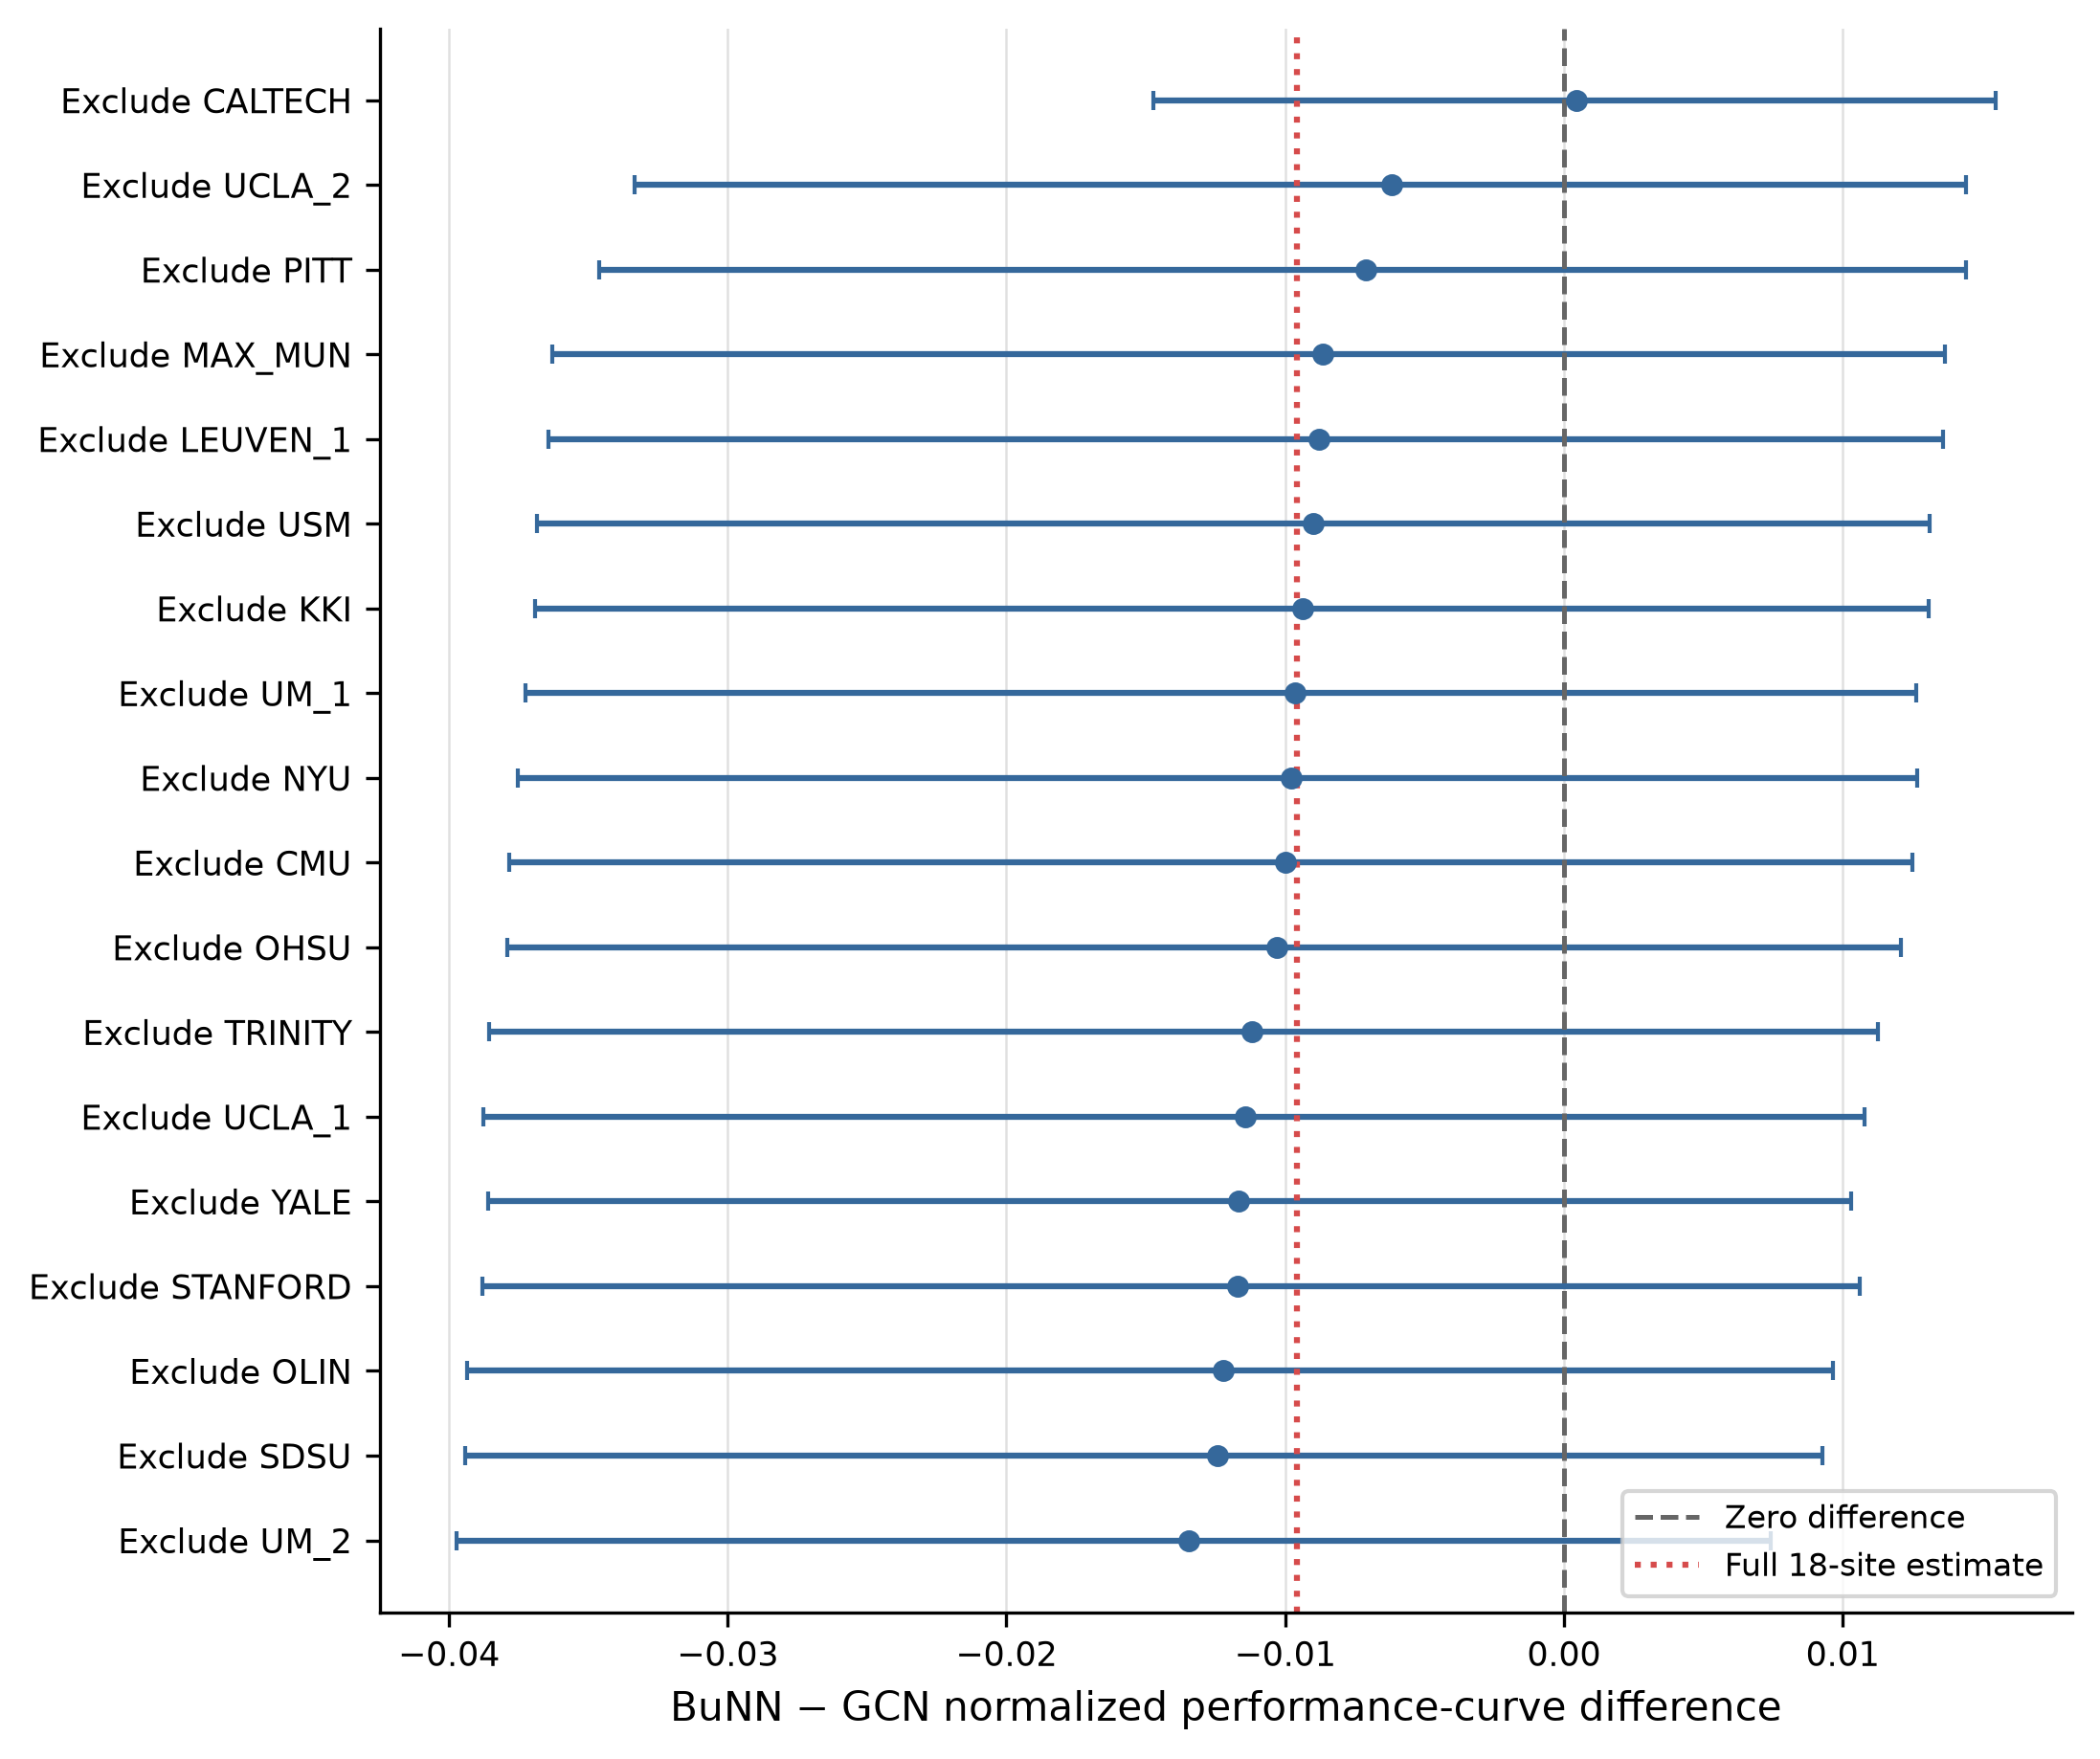
\includegraphics[width=0.92\textwidth]{site_influence.png}
  \caption{Leave-one-site influence on the BuNN--GCN curve contrast. This
  analysis tests whether the confirmatory average is driven by a single site;
  it does not create 18 independent replications.}
  \label{fig:site-influence}
\end{figure}

\begin{figure}[htbp]
  \centering
  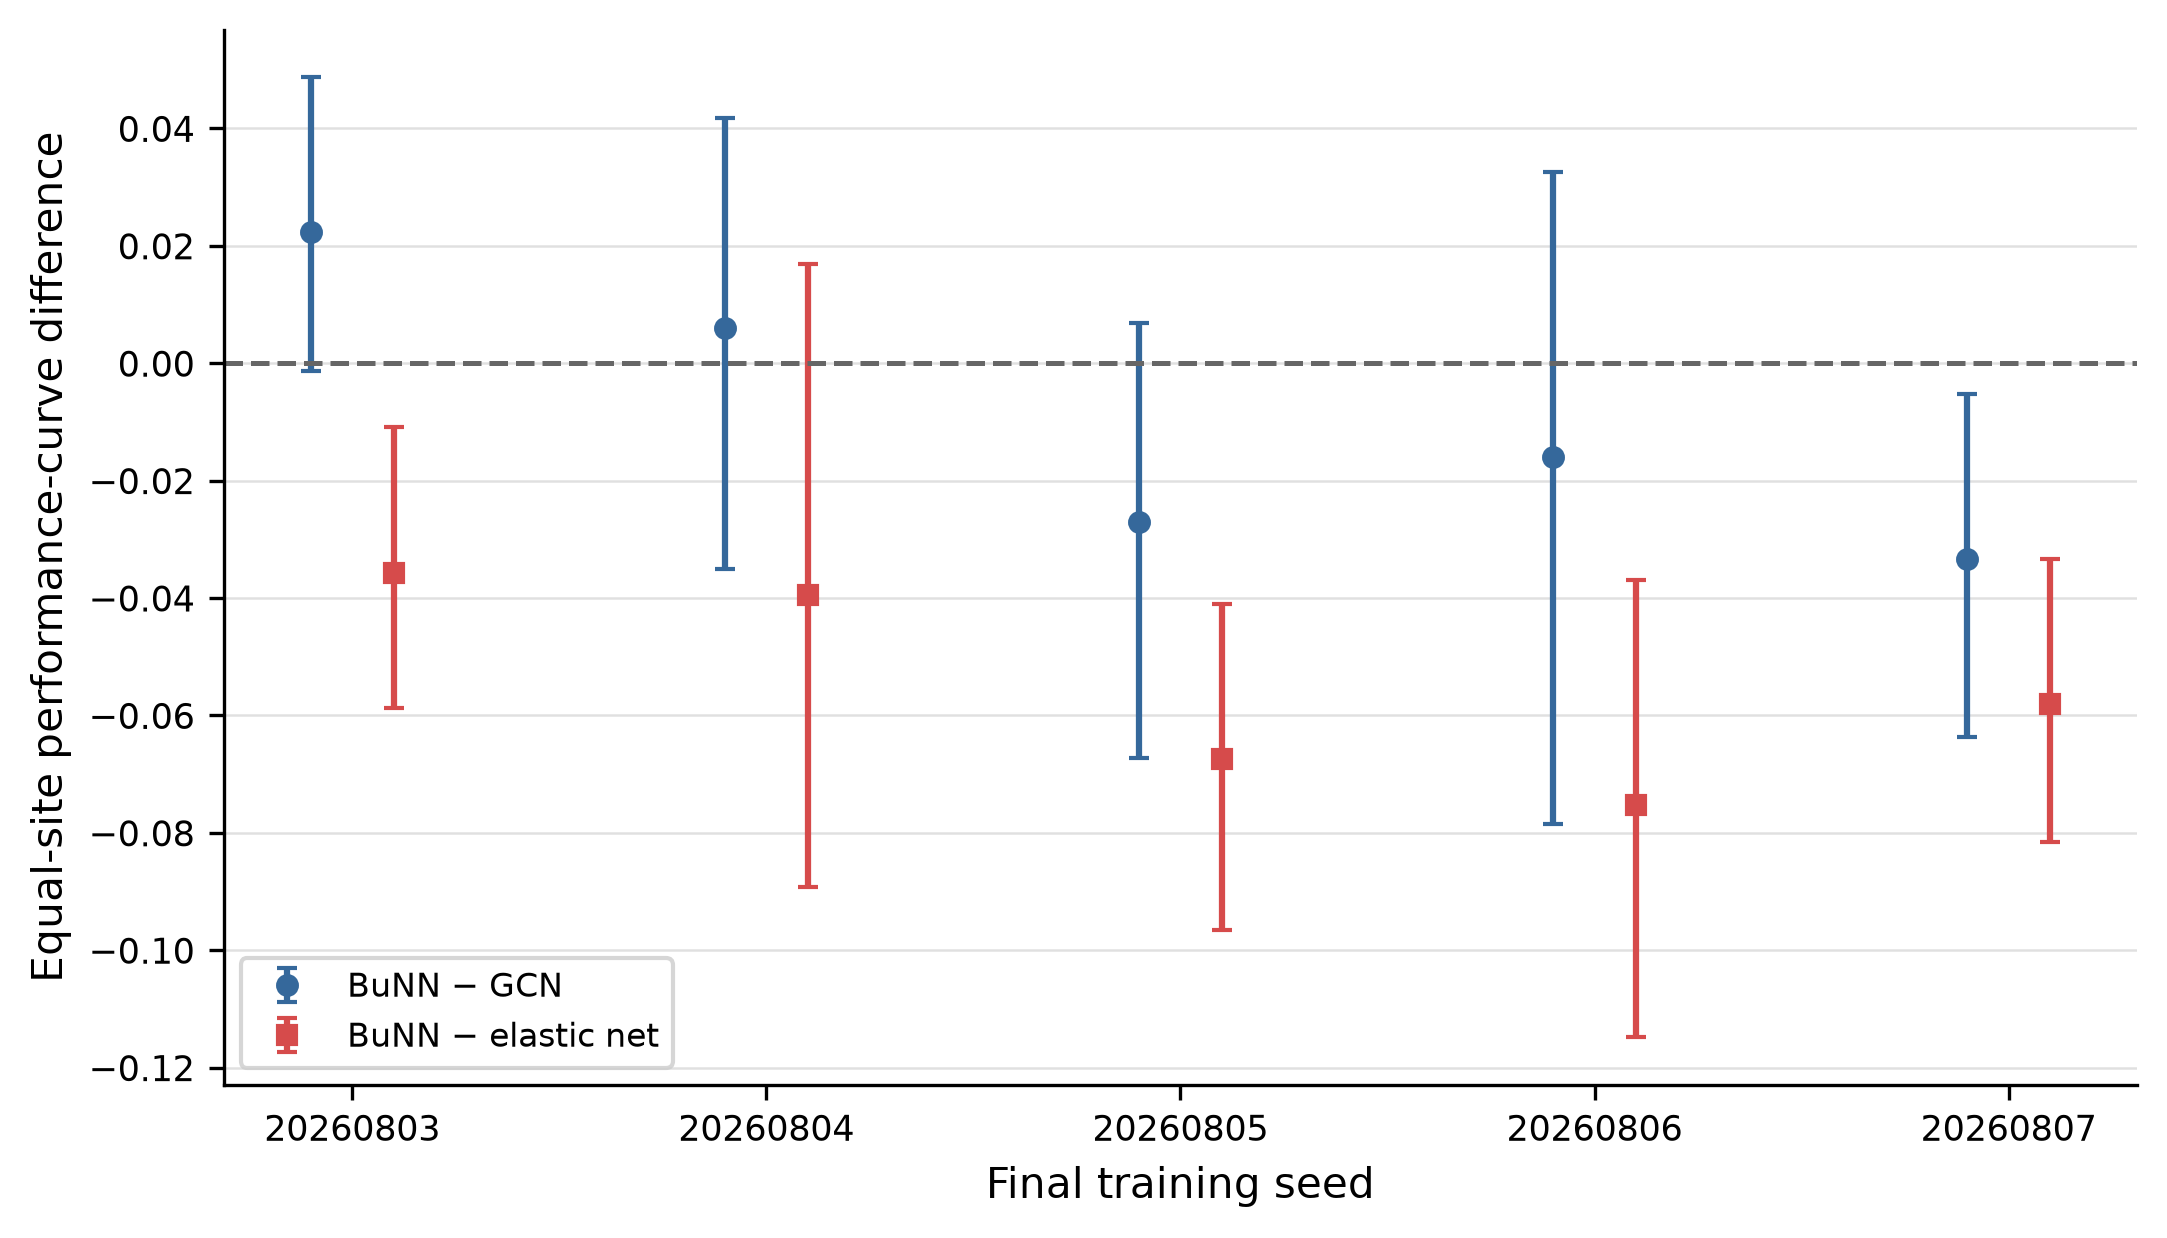
\includegraphics[width=0.88\textwidth]{seed_stability.png}
  \caption{BuNN--GCN contrast across the five fixed final training seeds.
  Variation across seeds shows that the small average difference is sensitive
  to optimization randomness.}
  \label{fig:seed-stability}
\end{figure}

\subsection{Execution cost}

Learned BuNN used 8,529 parameters, compared with 5,889 for GCN. Across the
recorded fits, BuNN required 31.14 total fit-hours and GCN required 15.09.
Maximum recorded peak GPU memory remained below 0.38 GiB for both. The low
memory use reflects small graphs and models; the workload was dominated by
many independent fits rather than a single large tensor. Runtime figures are
specific to this implementation and the A10G system.

\begin{table}[htbp]
\centering
\caption{Observed operator cost and equal-site curve performance.}
\label{tab:efficiency}
\small
\begin{tabularx}{\textwidth}{@{}Y r r r r@{}}
\toprule
\textbf{Operator} & \textbf{Parameters} & \textbf{Fit-hours} & \textbf{Peak GPU GiB} & \textbf{Curve BA} \\
\midrule
GCN & 5,889 & 15.09 & 0.373 & 0.5945 \\
Trivial bundle & 5,889 & 25.99 & 0.377 & 0.5911 \\
Learned BuNN & 8,529 & 31.14 & 0.378 & 0.5849 \\
\bottomrule
\end{tabularx}
\end{table}

\section{Discussion}

The proposed BuNN advantage did not carry into this ABIDE-I pipeline. Learned
bundle transport did not improve the performance--density curve over GCN,
did not beat the strongest regularized connectome baseline, and did not
preserve matched-anchor effective rank more strongly. Because inputs,
backbone, tuning budget, and operator controls were held fixed, the result
speaks directly to this propagation design rather than to a broad comparison
of unrelated models.

The intervention audit resolves one ambiguity in that negative comparison.
BuNN's learned maps were not ignored: replacing them with random orthogonal
maps caused a large, multiplicity-controlled loss of held-out performance.
The failure to beat GCN or the elastic net therefore cannot be explained by
saying that training never used the map system. Instead, computationally
important learned transformations existed inside a model whose overall
inductive bias still did not improve cross-site prediction.

\subsection{Why the result was plausible before the experiment}

The original hypothesis was not arbitrary. Ordinary diffusion can contract
node representations, while orthogonal transport can align features before
averaging. In graph problems where neighboring features are expressed in
different useful frames, that operation can protect structure that direct
averaging would erase. BuNN theory and prior synthetic evaluations therefore
provided a reasonable architectural motivation \cite{bamberger2025bundle}.

The experiment nevertheless placed that idea in an unusually demanding
setting. Functional connectomes are dense, and the node feature is already a
global profile. The benefit of transporting locally available information may
be small when every node already describes its relationship with all other
nodes.

\subsection{What the completed evidence can explain}

The data support a layered explanation, not a single proven mechanism.

\begin{table}[htbp]
\centering
\caption{Evidence-based interpretation of the null result.}
\label{tab:explanation}
\small
\begin{tabularx}{\textwidth}{@{}p{3.1cm}Y Y@{}}
\toprule
\textbf{Observation} & \textbf{Supported interpretation} & \textbf{What it does not prove} \\
\midrule
Diffusion curves decline with density & Adding more propagation edges is associated with worse held-out-site prediction in this pipeline. & A universal law of over-smoothing or a causal biological mechanism. \\
BuNN does not beat GCN & Learned transport provides no detected predictive advantage over ordinary aggregation here. & That BuNN never works on brain or non-brain graphs. \\
BuNN remains below elastic net & A regularized model on the full connectome is the stronger practical reference for these inputs. & That nonlinear modeling is always unnecessary. \\
Learned-local anchor already has high raw rank & Extra node-wise map capacity can create an apparent raw diversity advantage without transport. & That every aspect of the learned maps is useless. \\
Matched-anchor rank favors GCN & The proposed common-frame representation-preservation advantage is not supported. & A causal mediation pathway from rank to prediction. \\
Random maps reduce BA by 8.86 points & Accepted predictions depend on properties of the learned map system. & Biological bundle geometry or causal neural transport. \\
Map shuffling has a smaller effect & The learned map collection matters more than the exact node assignment under this intervention. & That node identity is irrelevant in every architecture. \\
Degree-preserving rewiring reduces BA by 1.23 points & The constructed propagation graph contributes modestly to prediction. & Anatomical validity of the graph or a universal topology effect. \\
Diagnostic--performance correlations are weak & Large representation changes do not reliably co-vary with predictive changes across site-density cells. & Proof that representations can never mediate prediction. \\
Site and seed sensitivity & The small BuNN--GCN difference is not stable to all reasonable weighting and optimization choices. & That the full result is invalid or that site effects explain every difference. \\
\bottomrule
\end{tabularx}
\end{table}

The strongest current explanation is therefore architectural and data-based.
The full connectivity rows already expose global information, while denser
propagation averages those profiles. Learned orthogonal maps materially shape
BuNN's own predictions, but the much smaller topology-rewiring effect suggests
that message passing over the selected positive-edge graph contributes less.
The model can learn useful internal coordinate transformations without those
transformations outperforming a simpler GCN or a linear model that directly
uses the complete connectome. This interpretation fits both Study 1 and E1;
it is not a causal proof of which internal feature components were lost.

\subsection{Why the learned-local control matters}

BuNN introduces additional parameters through its map generator. A comparison
with GCN alone could credit transport for differences caused by that added
capacity. The learned-local control keeps the map generator but removes
inter-node diffusion. Its high zero-density effective rank shows how a naive
raw-embedding analysis could overstate preservation. Anchoring each operator
to its corresponding no-propagation state makes the mechanism comparison more
credible.

\subsection{Site heterogeneity and uncertainty}

The primary BuNN--GCN confidence interval crossed zero, and participant
weighting reversed the point-estimate sign. Individual site exclusions and
training seeds changed the magnitude and sometimes the direction of this
small difference. The correct conclusion is not that the models are exactly
equivalent. It is that no BuNN advantage was detected and that a gain of 0.03
balanced accuracy on the pre-specified curve estimand is inconsistent with
the observed upper confidence bound.

The contrast against the connectome elastic net is more stable. Its interval
remained below zero, indicating that the learned BuNN curve underperformed the
regularized non-graph reference in this analysis. That is an important result
because a paper comparing only neural graph variants could miss the strongest
available baseline.

\subsection{Limitations}

The conclusions are conditional on ABIDE-I, C-PAC filtered data without
global-signal regression, the AAL-116 atlas, Pearson correlations and Fisher
transformation, positive-edge propagation graphs, full connectivity-row node
features, the 0--20 percent density grid, the shared two-layer backbone, and
the fixed tuning budget. Other atlases, preprocessing pipelines, graph
construction rules, node features, or BuNN architectures may behave
differently.

The study uses observational functional associations. It cannot identify
anatomy, excitation, inhibition, or causal neural communication. The technical
quality-control rule does not remove demographic or clinical sampling bias.
Site sample sizes differ, and an equal-site mean answers a different question
from a participant-weighted mean. The representation diagnostics are
computational summaries; their association with prediction is not a causal
mediation analysis.

E1 was specified only after the Study 1 result was known, so it is a post-hoc
mechanistic audit rather than an independent confirmation. Its interventions
are deliberately artificial. Random maps can disrupt the coordinate system
expected by downstream learned weights, identity maps remove both learned
orientation and reflections, and node shuffling preserves the learned map
distribution while breaking its assignment. Their effect sizes reveal
functional dependence under these checkpoints, not the effect of changing a
single isolated biological mechanism. Finally, the completed report does not
contain an external ABIDE-II validation cohort.

\subsection{Remaining extensions and their evidential role}

The accepted-checkpoint intervention audit is now complete and independently
audited. It remains separate from the confirmatory result because its protocol
was frozen after Study 1 was known. Deeper matched GCN/BuNN networks, a
leakage-free Wang-style time-series model, synthetic ground-truth geometry,
and prospective ABIDE-II evaluation remain separate studies. They should not
be blended into either completed analysis or described as results until their
protocols and outputs are frozen and audited.

\section{Conclusion}

In this pre-specified ABIDE-I analysis, learned orthogonal bundle transport did
not improve the held-out-site performance--density curve over GCN. It also
failed to surpass identity propagation or the learned-local control and
remained below the regularized connectome baseline. Common-frame,
matched-anchor diagnostics did not support the proposed
representation-preservation advantage.

The finding does not show that bundle geometry is biologically false or that
BuNNs are generally ineffective. It shows something narrower and useful:
for dense functional-connectome graphs whose node features already contain
global connectivity information, this learned transport operator added
capacity and runtime without a detected advantage over GCN or elastic net.
The post-hoc checkpoint audit adds an important qualification. Learned maps
were computationally active: replacing them with random orthogonal maps
reduced balanced accuracy by 8.86 points after multiplicity-controlled
inference. Exact node-map placement and degree-preserving topology contributed
less, and representation changes were only weakly associated with prediction
changes.

The combined evidence therefore explains the negative comparison without
dismissing BuNN as inert. It learned consequential internal transformations,
but those transformations did not convert the selected graph and globally
informed features into better cross-site classification. That distinction is
the main contribution of the completed study. It was obtained through matched
controls, held-out-site evaluation, strong non-graph baselines, gauge-aware
diagnostics, frozen decision rules, checkpoint interventions, and independent
artifact audits.

\clearpage
\section*{Evidence Boundary and Remaining Work}
\addcontentsline{toc}{section}{Evidence Boundary and Remaining Work}

\begin{longtable}{@{}p{3.2cm}p{5.6cm}p{5.5cm}@{}}
\caption{Boundary between completed evidence and planned work.}\label{tab:status}\\
\toprule
\textbf{Component} & \textbf{Completed and audited} & \textbf{Not yet a result} \\
\midrule
\endfirsthead
\toprule
\textbf{Component} & \textbf{Completed and audited} & \textbf{Not yet a result} \\
\midrule
\endhead
Data & ABIDE-I C-PAC filtered, no-GSR AAL time series; technical QC; 754-person connectome archive. & Alternative preprocessing, atlases, negative-edge propagation, ABIDE-II. \\
Classical models & Covariate, connectome elastic-net, and combined baselines across all 18 held-out sites. & Additional harmonization or feature-selection families. \\
Neural models & Two-layer identity, learned-local, GCN, trivial-bundle, and learned-BuNN operator study; five seeds; complete density grid. & Five-layer matched study, Wang-inspired time-series architecture. \\
Mechanism evidence & Common-frame representation curves, matched anchors, site influence, seed stability, efficiency, and the audited 360-checkpoint map/topology intervention study. & Component-level feature-loss analysis and ground-truth synthetic geometry. \\
External validity & None claimed beyond the frozen ABIDE-I pipeline. & Prospective preprocessing-compatible ABIDE-II evaluation. \\
\bottomrule
\end{longtable}

\clearpage
\appendix
\section{Reproducibility Record}

The repository separates immutable scientific artifacts from presentation
files. Raw participant derivatives, checkpoints, and credentials are excluded
from the public release package. The report draws its numbers from generated
tables and macros tied to accepted analysis hashes. The following checks were
completed before the Study 1 result was interpreted:

\begin{itemize}
  \item all 18 outer sites were present;
  \item expected tuning, prediction, metric, diagnostic, and runtime row counts
  were complete;
  \item model and data contracts matched their frozen hashes;
  \item hidden metrics were independently recomputed before unblinding;
  \item parallel worker outputs matched the validated sequential execution in
  the engineering equivalence test;
  \item site-bootstrap and sign-flip analyses were built and tested on
  synthetic data before use on accepted results;
  \item report figures and tables were regenerated from the frozen result
  snapshot rather than edited manually.
\end{itemize}

The current source code, report source, manifests, and AI-use log are stored in
the project repository. Participant-level source data are not embedded in this
PDF.

\section{AI-Use Detail Required Before Submission}

The local AI-use ledger is more detailed than the summary in the front matter,
but a competition submission requires the researcher to verify it against
retained chats and product records. At minimum, the final disclosure should
state for every tool:

\begin{enumerate}
  \item product and model/version where known;
  \item dates or time period of use;
  \item stages of the research in which it was used;
  \item purposes and approximate frequency;
  \item files, decisions, or outputs affected;
  \item what the student independently checked; and
  \item whether prior supervisor approval was obtained.
\end{enumerate}

This completed evidence report does not invent missing Claude or Cursor history.
Those details must be supplied by the researcher.

\clearpage
\begin{singlespace}
\bibliographystyle{IEEEtran}
\bibliography{../references}
\end{singlespace}

\end{document}
